%!TEX root = ../../thesis.tex
\define{\chapterpath}{\allchapterspath/planning}
\define{\imgpath}{\chapterpath/img}

\define{\twoplanningwidth}{0.7}
\define{\threeplanningwidth}{1}
\define{\twotworldsize}{0.8}
\define{\threetworldsize}{1}
\define{\plotsize}{0.6}

\chapter{Planning upon Uncertainty}
\label{chapter:planning}
\minitoc


In previous chapter, we presented our algorithm allowing to solve a task from human instruction signals without knowing in advance the mapping between the signals and their meanings. We have seen seen that the performances of our system is affected by the action selection method used by our robot. In this section we investigate further how the agent should plan its action to improve the learning efficiency. To do so, our agent will look for action that disambiguate between hypothesis, which is the one that reduce the uncertainty about which hypothesis is the correct one.

We start by explaining what should be the method and measure of uncertainty use by a system that has access the the true signal to meaning mapping. We then providing an intuition on what are is the additional sources of uncertainty inherent to our problem, and link it with the problem of symmetries seen in chapter~\ref{chapter:lfui:symmetries}. After this, we propose two ways of estimating the uncertainty in our scenario, one on the signal space and one on the meaning space using hypothetic signals. We finally present simulated experiments showing that our measure of uncertainty allow the robot to plan efficiently its action in order to disambiguate between hypothesis. Those results uses a series of dataset of different qualities and dimensionality, and we will see that the performance of the system are affected by the quality of the data more than their dimensionality. An important aspect of our algorithm is to detect those cases it can not discriminate between task, and for those case where a good classifier can not be found, the algorithm will not select between hypothesis.

On this basis we will transition to chapter~\ref{chapter:bci} which present an application to brain computer interaction scenarios where human users guide an agent on a specific square of a grid using feedback signals and without having to calibrate the brain decoder before hand.

%%%%%%%%%%%%%%%%%%%%%%%%%%%%%%%%%%%%%%%%%%%%%%
%%%%%%%%%%%%%%%%%%%%%%%%%%%%%%%%%%%%%%%%%%%%%%
%%%%%%%%%%%%%%%%%%%%%%%%%%%%%%%%%%%%%%%%%%%%%%
%%%%%%%%%%%%%%%%%%%%%%%%%%%%%%%%%%%%%%%%%%%%%%
%%%%%%%%%%%%%%%%%%%%%%%%%%%%%%%%%%%%%%%%%%%%%%
\section{Uncertainty for known signal to meaning mapping}

If the true mapping between human communicate signals and their meaning is provided to the machine, and that it still has to identify the correct task between a finite set of task and has access to the interaction frame, the learning process is rather trivial. Indeed, in such case, the robot should only compares if what the meaning received from the human match well with what is expected from the given frame and a given task. If they match then we can increase the probability of such task, if they do not match we can decrease the probability.

The robot should therefore seek for the state-action pairs that maximally disambiguate between hypothesis. For example, if for one given state-action pair, half of the hypothesis expect a signal of meaning ``correct'' and the other half expect one of meaning ``incorrect''. By performing this action in that state, the system will rule out half of the hypothesis once the user will have provided its feedback. 

It is important for this process to be weighted by the current probability associated with each task hypothesis. Indeed once we have rules out half of the hypothesis, we should only focus on differentiating the remaining hypothesis. For this the robot should seek for a new state-action pair where the remaining hypothesis will disagree on the expected meaning from the teacher.

But this process is here describe in a way that is not realistic, our robot can not query any state-action pair, it can not teleport but rather should navigate through the all state space to be able to finally perform that state-action pair. And on its way to a specific state-action pair, it may already have received new information changing its current belief on the hypothesis probabilities.

A solution to this problem is to add exploration-bonuses for each state-action pair corresponding to the uncertainty associated to each state-action pair. The agent can then select its next action considering the full map of uncertainty. By seeing those exploration-bonuses as rewards in a reinforcement learning scenario the agent select the action that maximizes uncertainty reduction on the task in the long term. There are several efficient model-based reinforcement learning exploration methods that add an exploration bonus for states that might provide more learning gains. Several theoretical results show that these approaches allow to learn tasks efficiently \cite{brafman2003r,kolter2009near}. 



\todo{
Following our notation, we can define an uncertainty measure as the variance of the expected meaning for each task weighted by their current probability, for a specific state and action and the feedback frame:

\begin{eqnarray}
U(s,a) = weightedVariance(p(l = ``correct''| s, a, \xi), p(\xi))
\end{eqnarray}



\cite{lopes2009active}, if the classifier is known, equation \ref{eq:planningOneSignal} reduces to the one presented in \cite{macl11simul}}


This method works well if the machine has access to the true intended meaning of the user, which is not the case for us. We will now investigate what makes our problem different in terms of planning.

%%%%%%%%%%%%%%%%%%%%%%%%%%%%%%%%%%%%%%%%%%%%%%
%%%%%%%%%%%%%%%%%%%%%%%%%%%%%%%%%%%%%%%%%%%%%%
%%%%%%%%%%%%%%%%%%%%%%%%%%%%%%%%%%%%%%%%%%%%%%
%%%%%%%%%%%%%%%%%%%%%%%%%%%%%%%%%%%%%%%%%%%%%%
%%%%%%%%%%%%%%%%%%%%%%%%%%%%%%%%%%%%%%%%%%%%%%
\section{Where is the uncertainty}
\label{chapter:planning:where}


In order to exemplify the specificity of our problem in terms of planning we will rely again on our T world scenario and compare the effect of different action selection strategies. We remind that the user always wants the robot to reach the left edge (marked by G1) of the T.


Starting form the explanation in previous section, if the agent knew how to interpret the teaching signals, i.e. which signal corresponds to correct or incorrect feedback, the optimal action to differentiate between the two hypothesis (G1 and G2) would be to perform right and left actions in the top part of the T. However as the classifier is not given, the agent builds a different model for each hypothesis and ends-up in with symmetric interpretation of the signals which are both as valid (see Figure~\ref{fig:planningrightleft}) and do not allow to differentiate between hypothesis.

\begin{figure}[!ht]
  \centering
  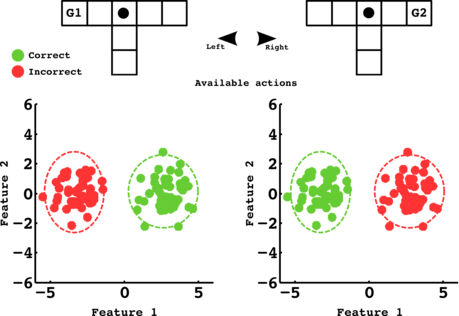
\includegraphics[width=\twotworldsize\columnwidth]{\visualspdf/tuto_feedback/Tworld_feedback_labeled_right_left_with_gaussian.pdf}
  \caption{Results of the labeling process if the agent only performs right and left actions in the top of the T world. This is the symmetry problem encountered in previous chapter~\ref{chapter:lfui:symmetries}. The resulting signal-label pairs for G1 and G2, while opposite, are both as likely to correspond to the data.}
  \label{fig:planningrightleft}
\end{figure}

Considering that the agent does not know the signal to meaning classifier, a sensitive option is to select actions that allow to unequivocally identify the model. In our scenario taking only up and down actions in the trunk of the T leads to identical interpretation for each hypothesis (see Figure~\ref{fig:planningupdown}). However this method do not allow to disambiguate between hypothesis and in most settings, such as the grid world we consider later, there is no state-action pair leading to unequivocal interpretations.

\begin{figure}[!ht]
  \centering
  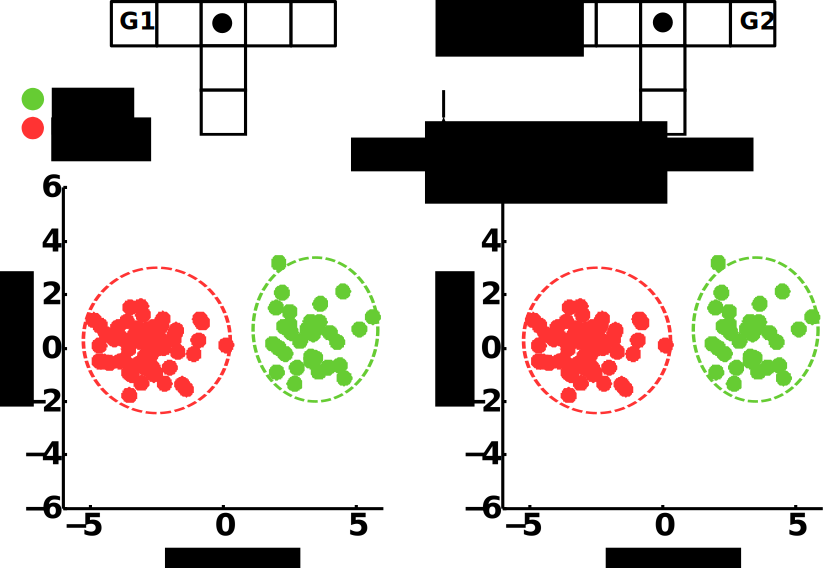
\includegraphics[width=\twotworldsize\columnwidth]{\visualspdf/tuto_feedback/Tworld_feedback_labeled_up_down_with_gaussian.pdf}
  \caption{Results of the labeling process if the agent only performs up and down actions in the trunk of the T. The interpretation of the signal for both hypothesis are the same, this method allow to build a good model.}
  \label{fig:planningupdown}
\end{figure}

Those two examples exemplify the specificity of our planning problem. The agent can not just try to differentiate hypothesis by finding state-action pair where expected feedback differs (left-right actions in Figure~\ref{fig:planningrightleft}) but should also collect data to build a good model (up-down actions in Figure~\ref{fig:planningupdown}). What is the optimal next action to take in the previous condition?

\begin{itemize}
\item In the situation from Figure~\ref{fig:planningrightleft}, the robot as a symmetric interpretation for G1 and G2 and should therefore perform an action that break this symmetry and collect one signal with identical label for both hypothesis. By performing the action down in the T trunk, both hypothesis will associated to the corresponding teaching signal a label ``incorrect'', which will break the symmetry.
\item In the situation from Figure~\ref{fig:planningupdown}, the robot as an identical interpretation for G1 and G2 and should therefore collect one signal whose label will be different for each hypothesis. By performing the action left in the top of the T, hypothesis G1 will associate the label ``correct'', while hypothesis will associate the label ``incorrect'', which will break the similarity between models.
\end{itemize}

Can we find a measure of uncertainty that account for both cases? The measure defined in previous section would not work as the uncertainty measure was independent of the signal-to-meaning mapping. Indeed this mapping was the same for every hypothesis. However in our scenario, each hypothesis has a different signal-to-meaning mapping and therefore there is also uncertainty on the signal-to-meaning mapping.

% \begin{itemize}
% \item In the situation from Figure~\ref{fig:planningrightleft}, when going left both hypothesis agree that they will receive a signal in the right part of the feature space even if they disagree on its meaning. However for action down, both hypothesis agree they should receive a signal of meaning ``incorrect'' but disagree on the expected location of such signal in the feature space.
% \item In the situation from Figure~\ref{fig:planningupdown}, when going down both hypothesis agree they will receive a signal in the left part of the feature space and agree on its meaning. However for action left, both hypothesis disagree about the meaning of the signal they should receive and as both share the same signal model they expect a signal in different locations of the feature space.
% \end{itemize}

We should measure uncertainty taking into account the uncertainty related to the different tasks, as well as, the uncertainty from the different interpretation models associated to each task. This characteristic will be visually exemplified in the next section and we will present two ways of measuring the uncertainty. The first method measures the uncertainty on the expected signals between each hypothesis for a given state-action pair. The second method present one signal sample to be evaluated by each hypothetic classifier an compared to the expectation from the state-action pair, we then measure the variance between the expectation of this signal sample between each hypothesis.


%%%%%%%%%%%%%%%%%%%%%%%%%%%%%%%%%%%%%%%%%%%%%%
%%%%%%%%%%%%%%%%%%%%%%%%%%%%%%%%%%%%%%%%%%%%%%
%%%%%%%%%%%%%%%%%%%%%%%%%%%%%%%%%%%%%%%%%%%%%%
%%%%%%%%%%%%%%%%%%%%%%%%%%%%%%%%%%%%%%%%%%%%%%
%%%%%%%%%%%%%%%%%%%%%%%%%%%%%%%%%%%%%%%%%%%%%%
\section{How can we measure this uncertainty}
\label{chapter:planning:how}

Before providing visual examples and associated equations to our uncertainty measure methods, we remind the importance of weighting the importance of each hypothesis proportional to their current probability. We then present our two methods, the first method measures the uncertainty on the expected signals between each hypothesis for a given state-action pair. The second method rely on sampling some teaching signals and asking each hypothesis if this signal is expected or not for the given state-action pair.

\subsection{The importance of weighting}

We want to measure the uncertainty about the tasks and signal models in order to collect information allowing to reduce this uncertainty. The uncertainty is therefore not a constant, it depends on our current belief about each hypothesis which changes whenever a new teaching signal is observed.

As we want to find which task is the correct one among the set of task hypothesis, we should aim a pulling apart the hypothesis which are currently the more probable. Once we have rules out half of the hypothesis, we should only focus on differentiating the remaining hypothesis. Therefore when estimating the uncertainty, we should weight each vote according to each hypothesis probability. In practice, if one hypothesis has a probability of 1 there should be no uncertainty for all state-action pairs considered.

\subsection{Measure on the signal space}

As detailed in section~\ref{chapter:planning:where}, our uncertainty measure should take into account the difference between the signal models associated to each hypothesis. We illustrate here in more details how this uncertainty can be measure by comparing the expected signals for each hypothesis.

We start by considering the situation in Figure~\ref{fig:planningrightleft} where the two hypothesis have symmetric signal models. As depicted in Figure~\ref{fig:uncertaintysignalrightleftagree}, when selecting action left, both hypothesis agree that they will receive a signal in the right part of the feature space even if they disagree on its meaning. Therefore taking action left in state 3 has low uncertainty on the expected signal.

\begin{figure}[!ht]
  \centering
  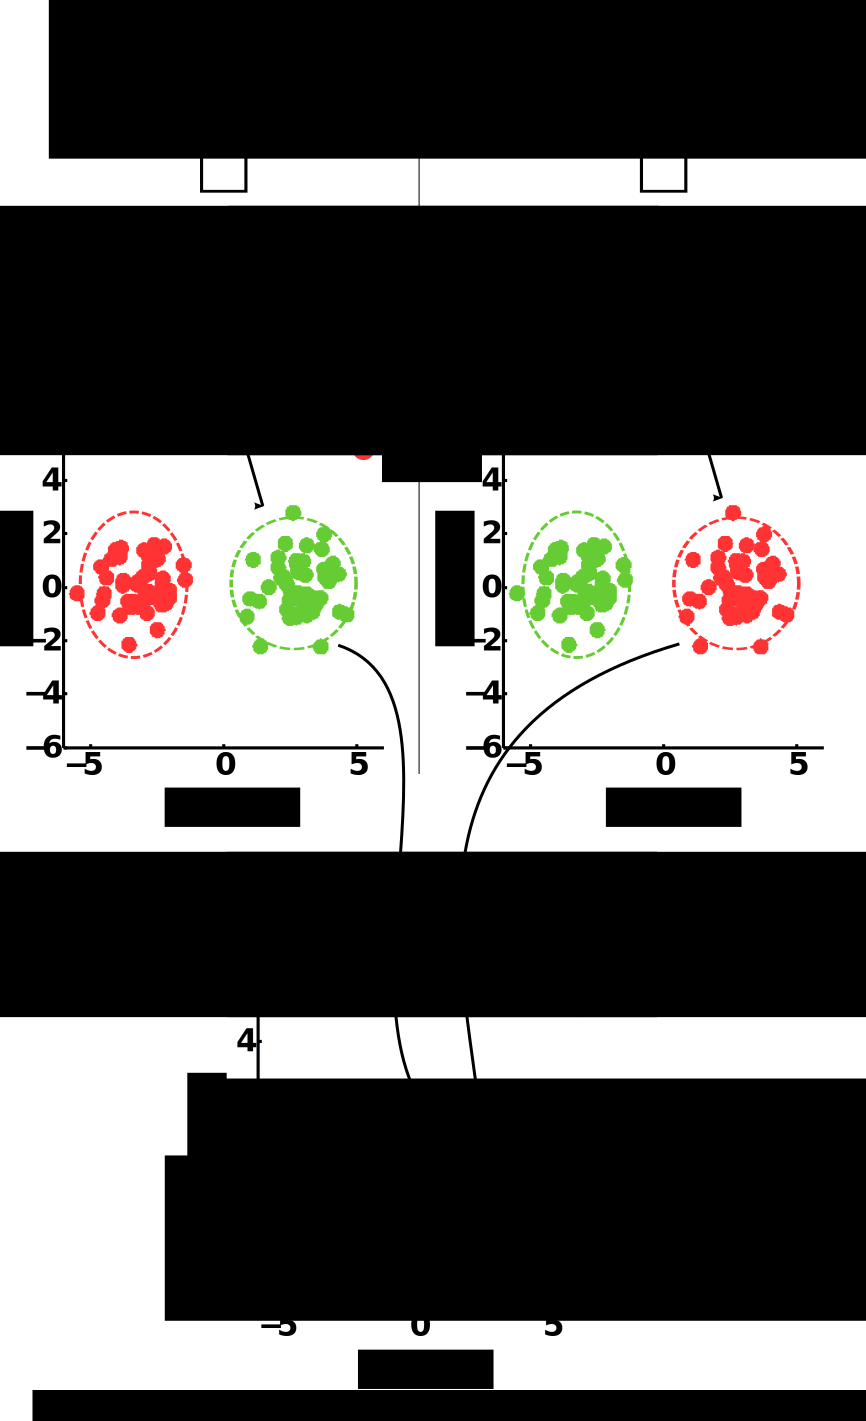
\includegraphics[width=\twoplanningwidth\columnwidth]{\visualspdf/planning/planning_right_left_agree.pdf}
  \caption{Expected signal for both hypothesis if agent performs action left in state 3 and given they currently have a symmetric interpretation of signals from Figure~\ref{fig:planningrightleft}. Both hypothesis expect the same signal, therefore there is no uncertainty associated to this state-action pair and the agent should not select this action in order to disambiguate between hypothesis.}
  \label{fig:uncertaintysignalrightleftagree}
\end{figure}

However for action down, both hypothesis agree they should receive a signal of meaning ``incorrect'' but disagree on the expected location of such signal in the feature space (see Figure~\ref{fig:uncertaintysignalrightleftdisagree}).Therefore taking action down in state 3 has high uncertainty on the expected signal.

\begin{figure}[!ht]
  \centering
  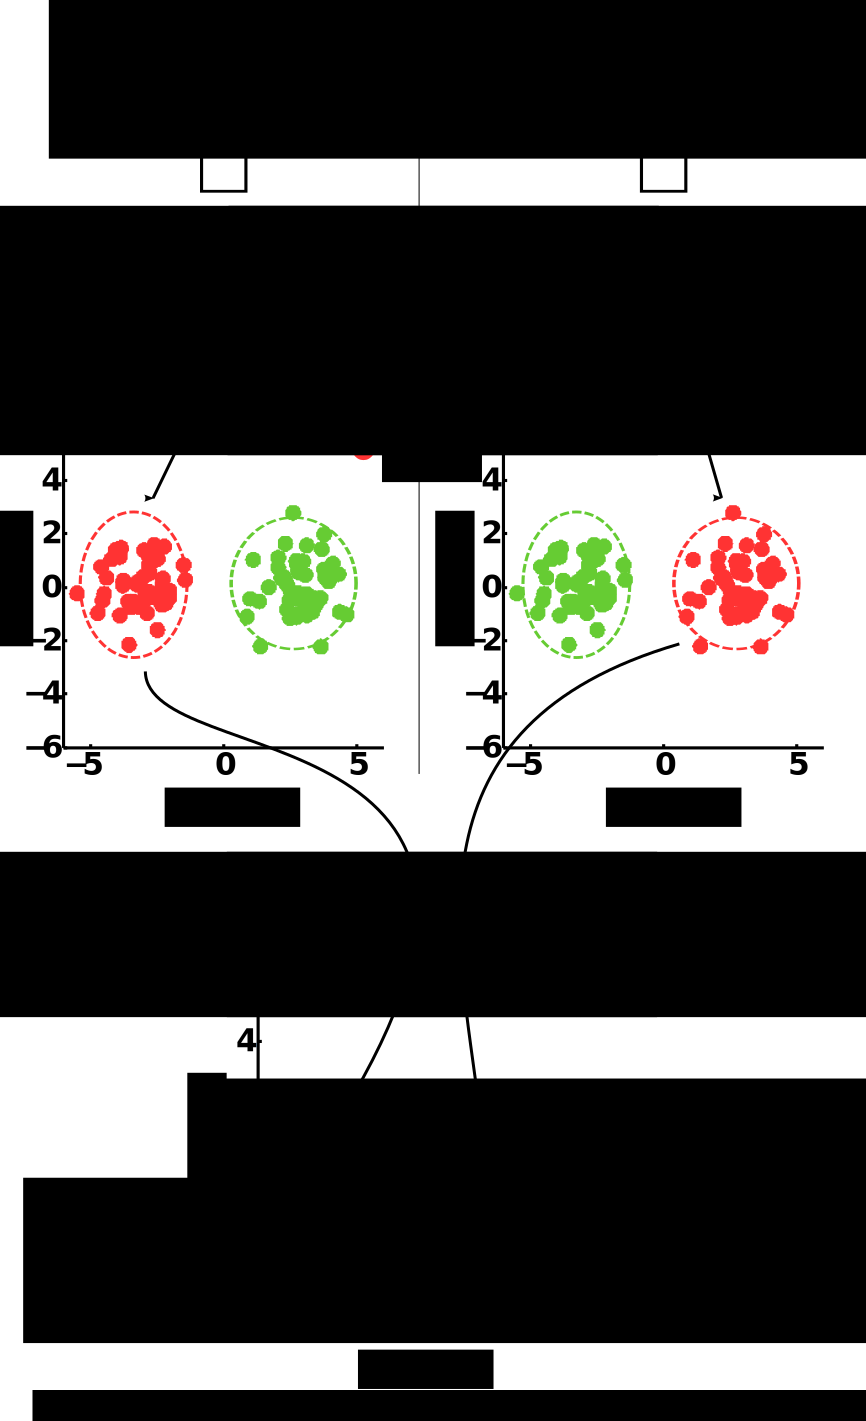
\includegraphics[width=\twoplanningwidth\columnwidth]{\visualspdf/planning/planning_right_left_disagree.pdf}
  \caption{Expected signal for both hypothesis if agent performs action down in state 3 and given they currently have a symmetric interpretation of signals from Figure~\ref{fig:planningrightleft}. The two hypothesis expect two different signals, therefore there is high uncertainty associated to this state-action pair and the agent should better perform this action in order to disambiguate between hypothesis.}
  \label{fig:uncertaintysignalrightleftdisagree}
\end{figure}


We now consider the situation in Figure~\ref{fig:planningupdown} where the two hypothesis have the same signal model. As depicted in Figure~\ref{fig:uncertaintysignalupdownagree}, when going down both hypothesis agree they will receive a signal in the left part of the feature space and agree on its meaning. Therefore taking action down in state 3 has low uncertainty on the expected signal.

\begin{figure}[!ht]
  \centering
  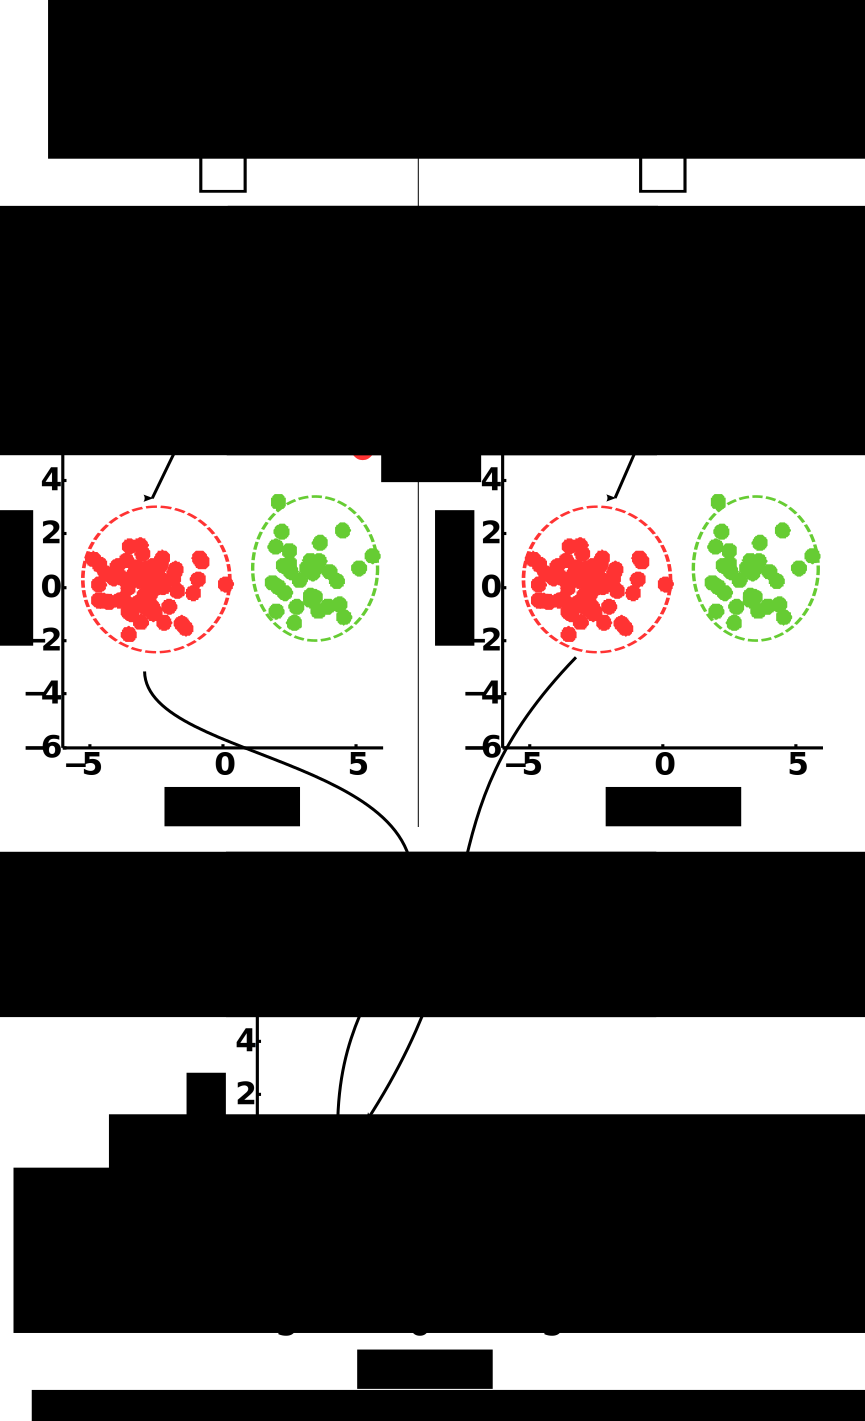
\includegraphics[width=\twoplanningwidth\columnwidth]{\visualspdf/planning/planning_up_down_agree.pdf}
  \caption{Expected signal for both hypothesis if agent performs action down in state 3 and given they currently have a similar interpretation of signals from Figure~\ref{fig:planningupdown}. Both hypothesis expect the same signal, therefore there is no uncertainty associated to this state-action pair and the agent should not select this action in order to disambiguate between hypothesis.}
  \label{fig:uncertaintysignalupdownagree}
\end{figure}

However for action left, both hypothesis disagree about the meaning of the signal they should receive and as both share the same signal model they expect a signal in different locations of the feature space (see Figure~\ref{fig:uncertaintysignalupdowndisagree}). Therefore taking action left in state 3 has high uncertainty on the expected signal.

\begin{figure}[!ht]
  \centering
  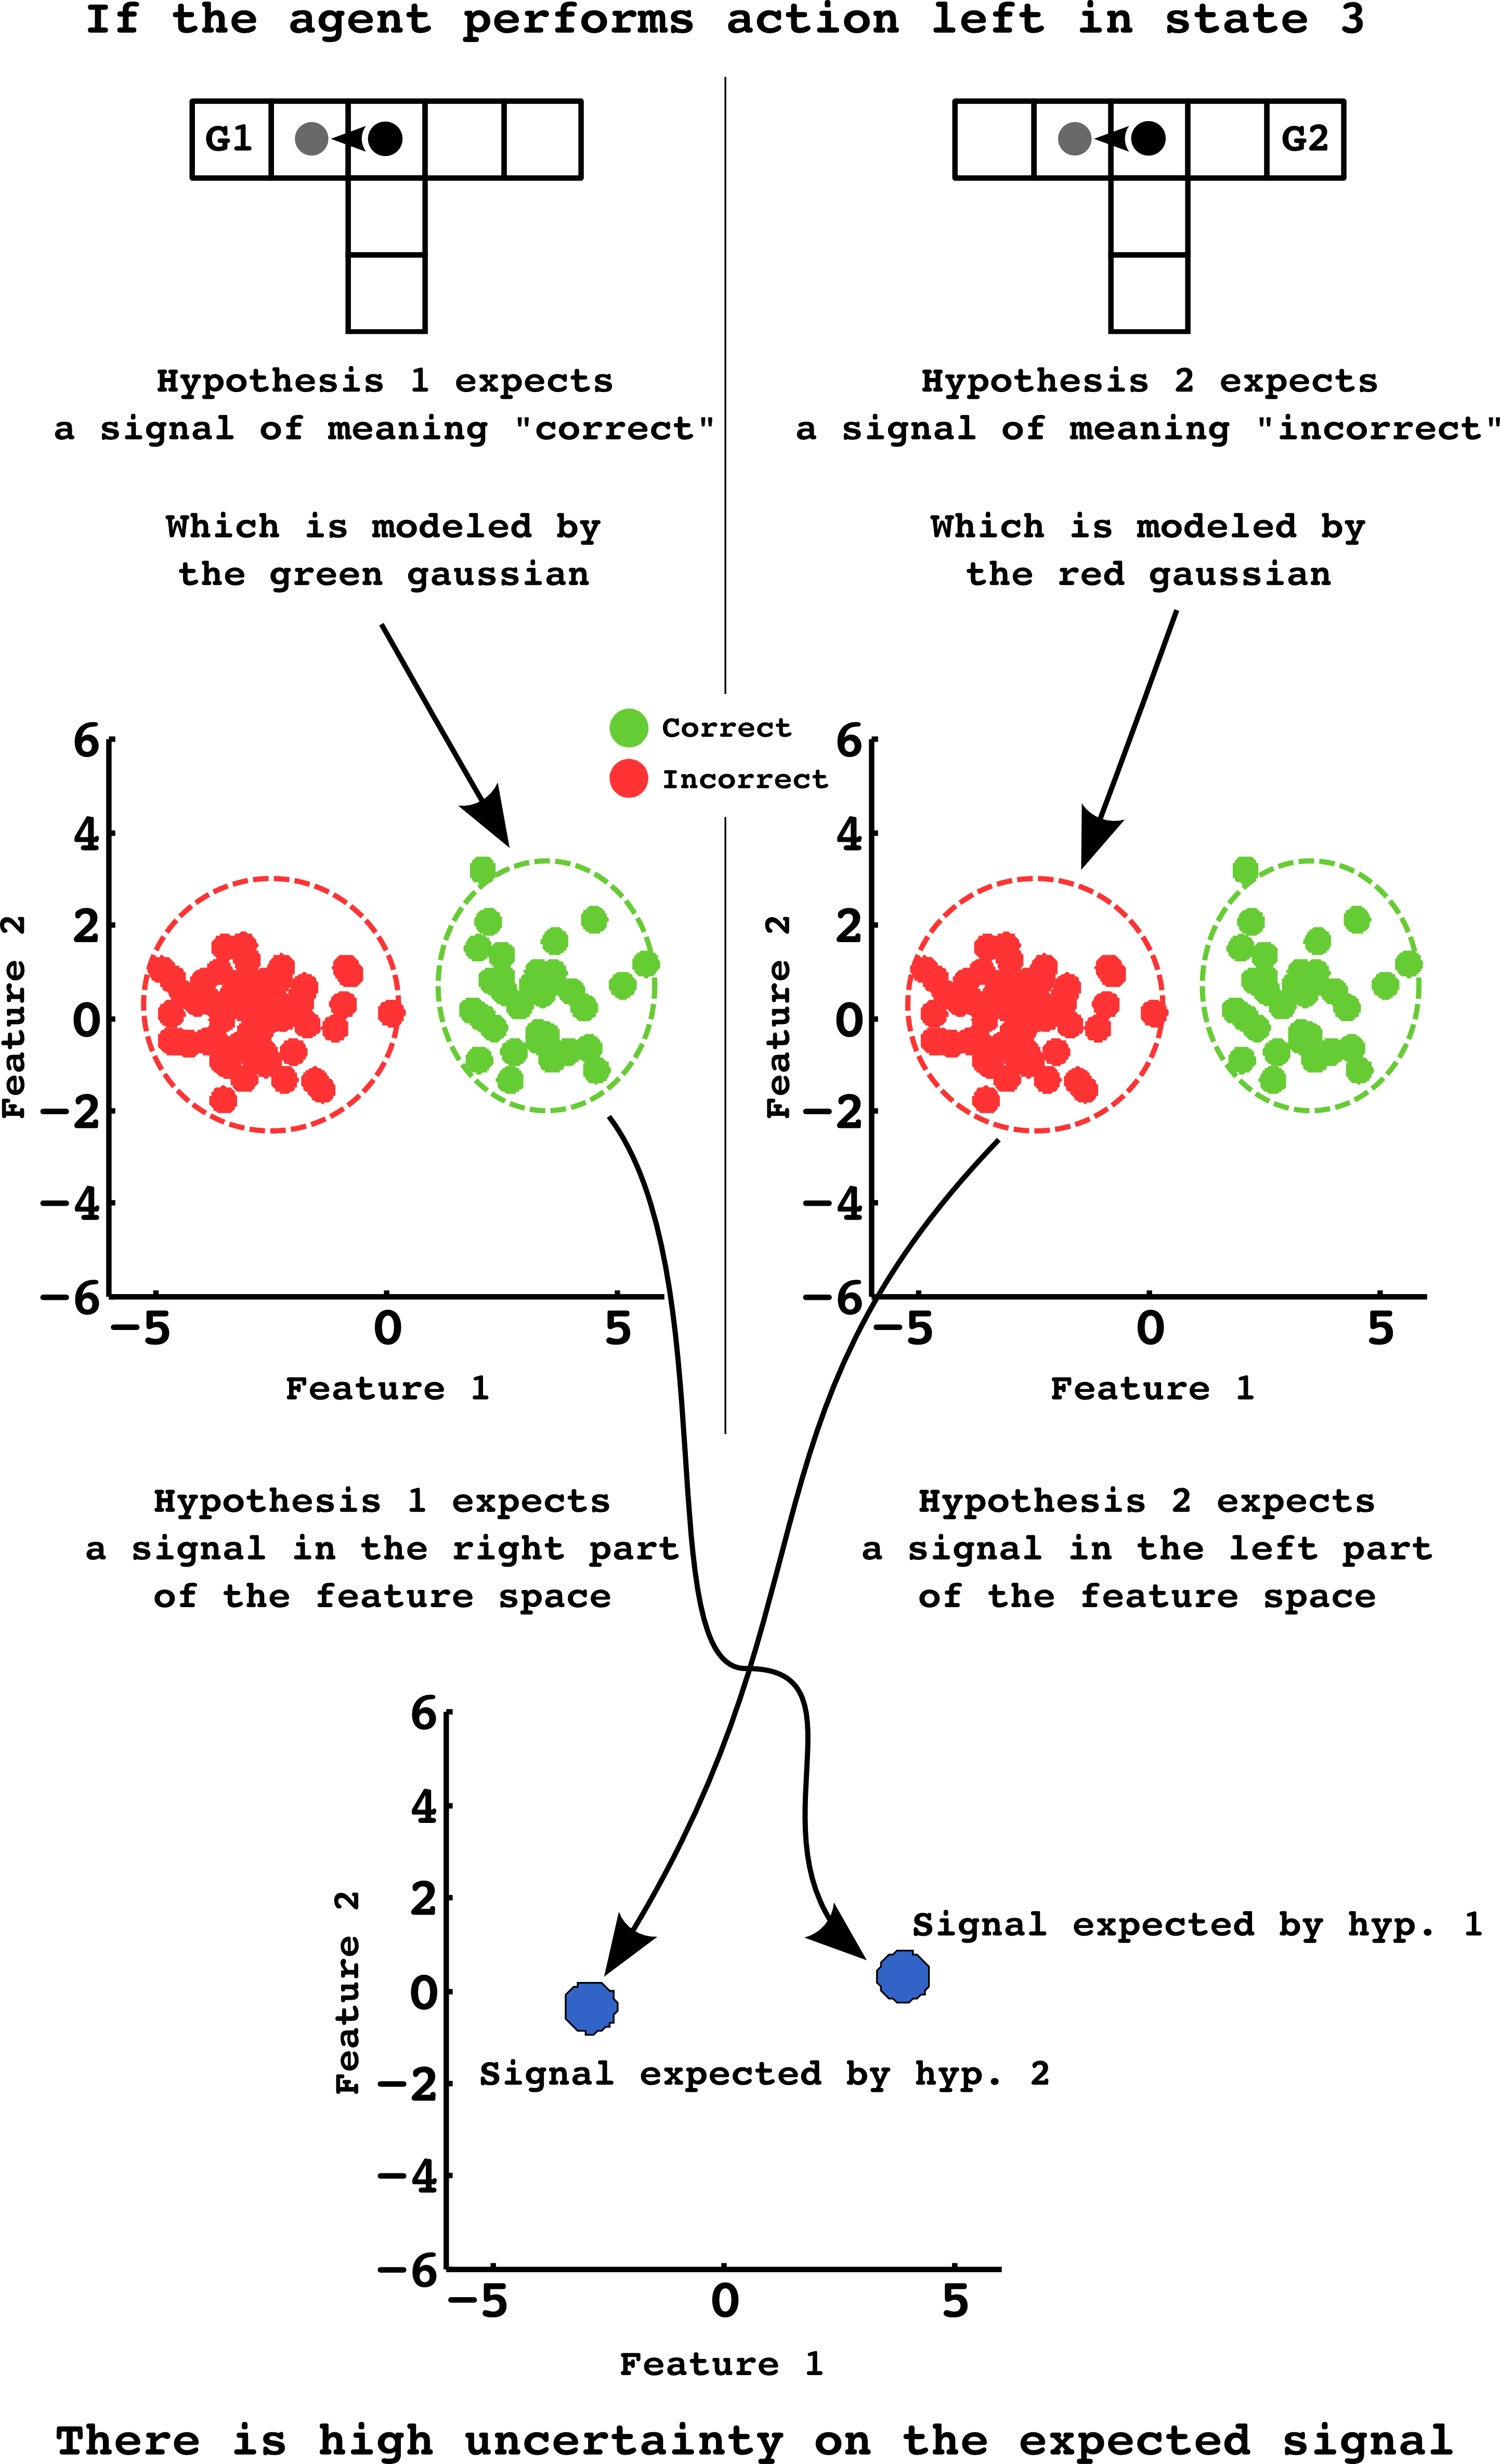
\includegraphics[width=\twoplanningwidth\columnwidth]{\visualspdf/planning/planning_up_down_disagree.pdf}
  \caption{Expected signal for both hypothesis if agent performs action left in state 3 and given they currently have a similar interpretation of signals from Figure~\ref{fig:planningupdown}. The two hypothesis expect two different signals, therefore there is high uncertainty associated to this state-action pair and the agent should better perform this action in order to disambiguate between hypothesis.}
  \label{fig:uncertaintysignalupdowndisagree}
\end{figure}


To sum up a state-action pair where the optimal actions and the signal models are the same for all hypotheses is unlikely to tell those hypothesis apart. It will be less informative that any other state-action where either optimal actions or signal models differ between hypotheses. To do so, for a given state-action pair, we should compute the similarity between the expected signals for each task. The more they are similar the less they are uncertain.

Our visual examples represent the expected signal for each hypothesis as the mean of the distribution corresponding to the expected label. This is a very rough approximation, indeed, the signal model is here model by a Gaussian distribution. Therefore comparing the similarity between the respective distribution would be more suited. Moreover, very often the frame take into account possible teaching mistake from the user and some probability of receiving an ``incorrect'' feedback while the action was optimal exist. This should also be taken into account when computing the similarity between signal distributions, which should in this example composed of mixture of Gaussian whose associated weight are the probability of receiving their associated meaning. In addition, we here only consider two hypothesis, but as soon as this number increases, we should compute the similarity between a multitude of distributions. 

We define a measure of global uncertainty $U(s,a)$ that is higher when, for a given state-action, there is a high incongruity between either optimal actions or signal models. For this we compute a similarity matrix $S$ where each element $S_{ij}(s,a)$ corresponds to the similarity of the distributions of signals associated to the expected label from tasks $i$ and $j$ if action $a$ is performed in state $s$. The final uncertainty value $U(s,a)$ is computed as the opposite of the weighted sum of the similarity matrix elements:

\begin{eqnarray}
U(s,a) &=& - \sum_{i = 1}^{T} \sum_{j = 1}^{T} ~~ S_{ij}(s,a) ~ p(\xi_i) ~ p(\xi_j)
\end{eqnarray}

Computed for each state and action, this measure is then used as an exploration bonus to select sequences of actions that guide the agent towards states that better identify the desired task. We provide an example of planning using this method in chapter~\ref{chapter:limitations:overlap}, where we use the distance between distribution means as our measure of similarity.

\subsection{A measure projected in the meaning space}

Estimating uncertainty in the signal space as presented in the previous subsection is in practice very costly as it requires to compute, for every state-action pair, the overlap between many continuous probability distributions weighted by their respective expected contribution. In this subsection we present an other metric for computing the uncertainty which rely on our pseudo-likelihood metric defined in chapter~\ref{chapter:lfui:how}. This method rely on sampling some teaching signals and asking every hypothesis if each of those signals are expected or not for the given state-action pair. 

We start by considering the situation in Figure~\ref{fig:planningrightleft} where the two hypothesis have symmetric signal models. As depicted in Figure~\ref{fig:uncertaintymeaningrightleftexpectedleft}, when selecting action left in state 3 and if the user sends a signal in the right part of the feature space, both hypothesis agree that this particular signal is expected given this state-action pair. Hypothesis 1 expects a signal of meaning ``correct'', and the teacher signal is classified as being of class ``correct''. Hypothesis 2 expects a signal of meaning ``incorrect'' and the teacher signal is classified as being of class ``incorrect''. Therefore receiving this particular signal after taking action left in state 3 has low uncertainty.

\begin{figure}[!ht]
  \centering
  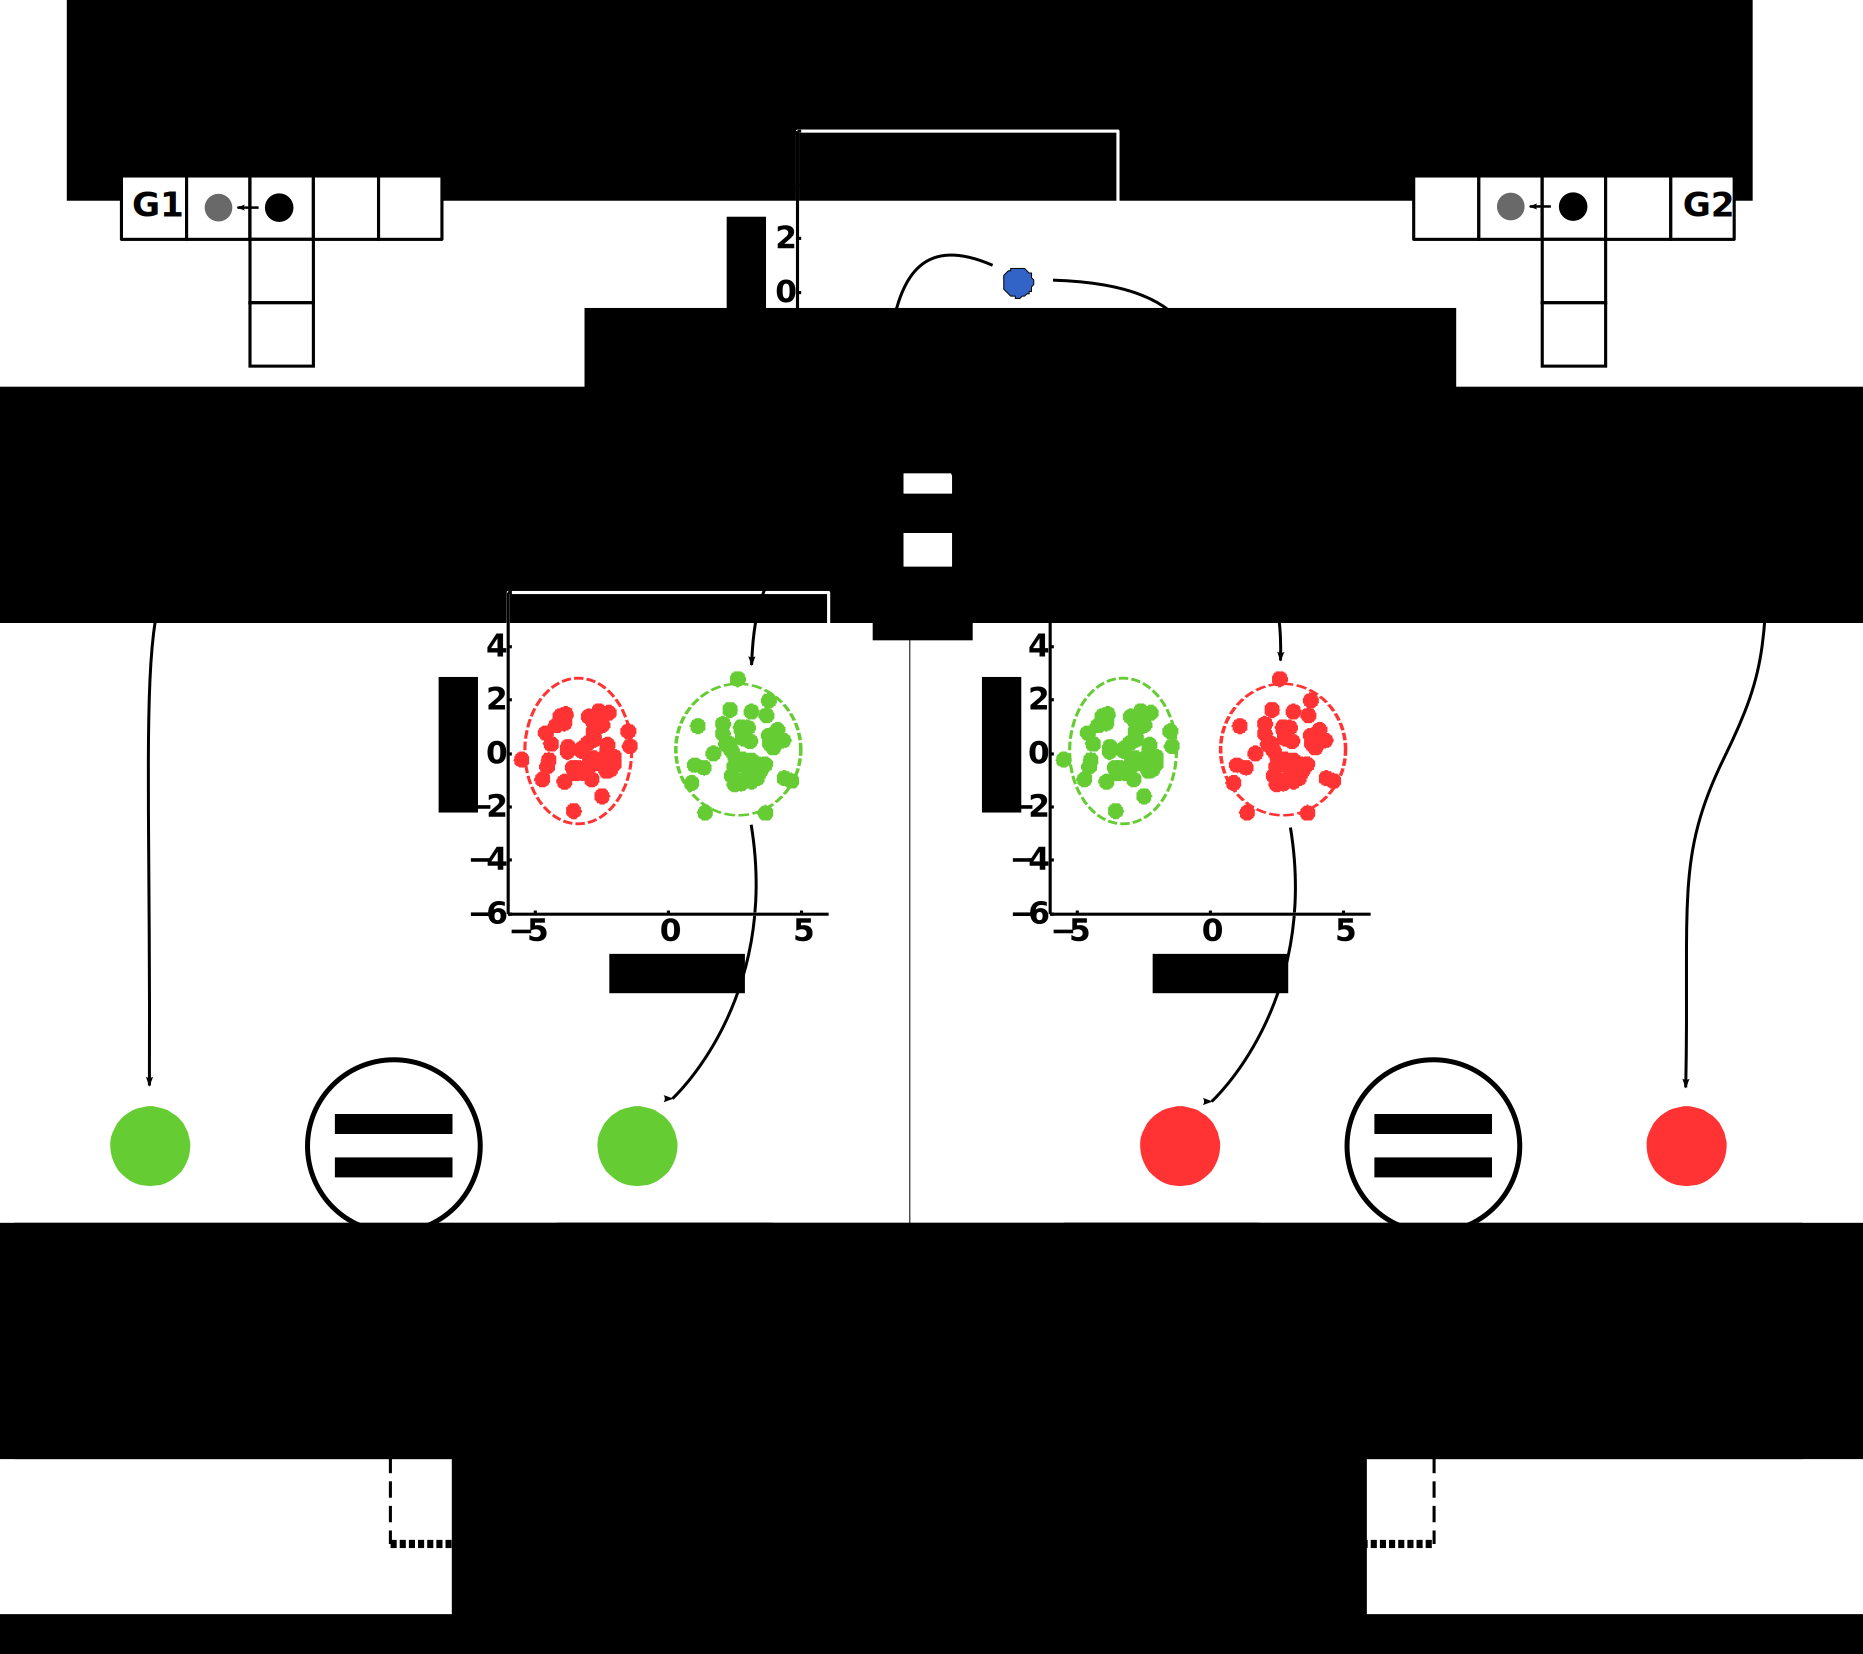
\includegraphics[width=\threeplanningwidth\columnwidth]{\visualspdf/planning/planning_right_left_expected_matched.pdf}
  \caption{Matching between expected labels and the prediction of a teaching signal sample on the right side of the feature space for the two hypothesis if the agent performs action left in state 3 and the two hypothesis currently have a symmetric interpretation of signals from Figure~\ref{fig:planningrightleft}. Both hypothesis agree that the label associated to a signal on the right side of the feature space match with the label predicted given the frame and the state-action pair considered. Therefore there is no uncertainty associated to this state-action pair and the agent should not select action left in order to disambiguate between hypothesis.}
  \label{fig:uncertaintymeaningrightleftexpectedleft}
\end{figure}

This same process can be executed for any teaching signal. For example, as depicted in Figure~\ref{fig:uncertaintymeaningrightleftexpectedright}, considering a teaching signal on the left side of the feature space, if the agent performs action left in state 3, both hypothesis agree that this particular signal is not expected. Hypothesis 1 expects a signal of meaning ``correct'', and the teacher signal is classified as being of class ``incorrect''. Hypothesis 2 expects a signal of meaning ``incorrect'' and the teacher signal is classified as being of class ``correct''. Therefore receiving this particular signal after taking action left in state 3 has low uncertainty.

\begin{figure}[!ht]
  \centering
  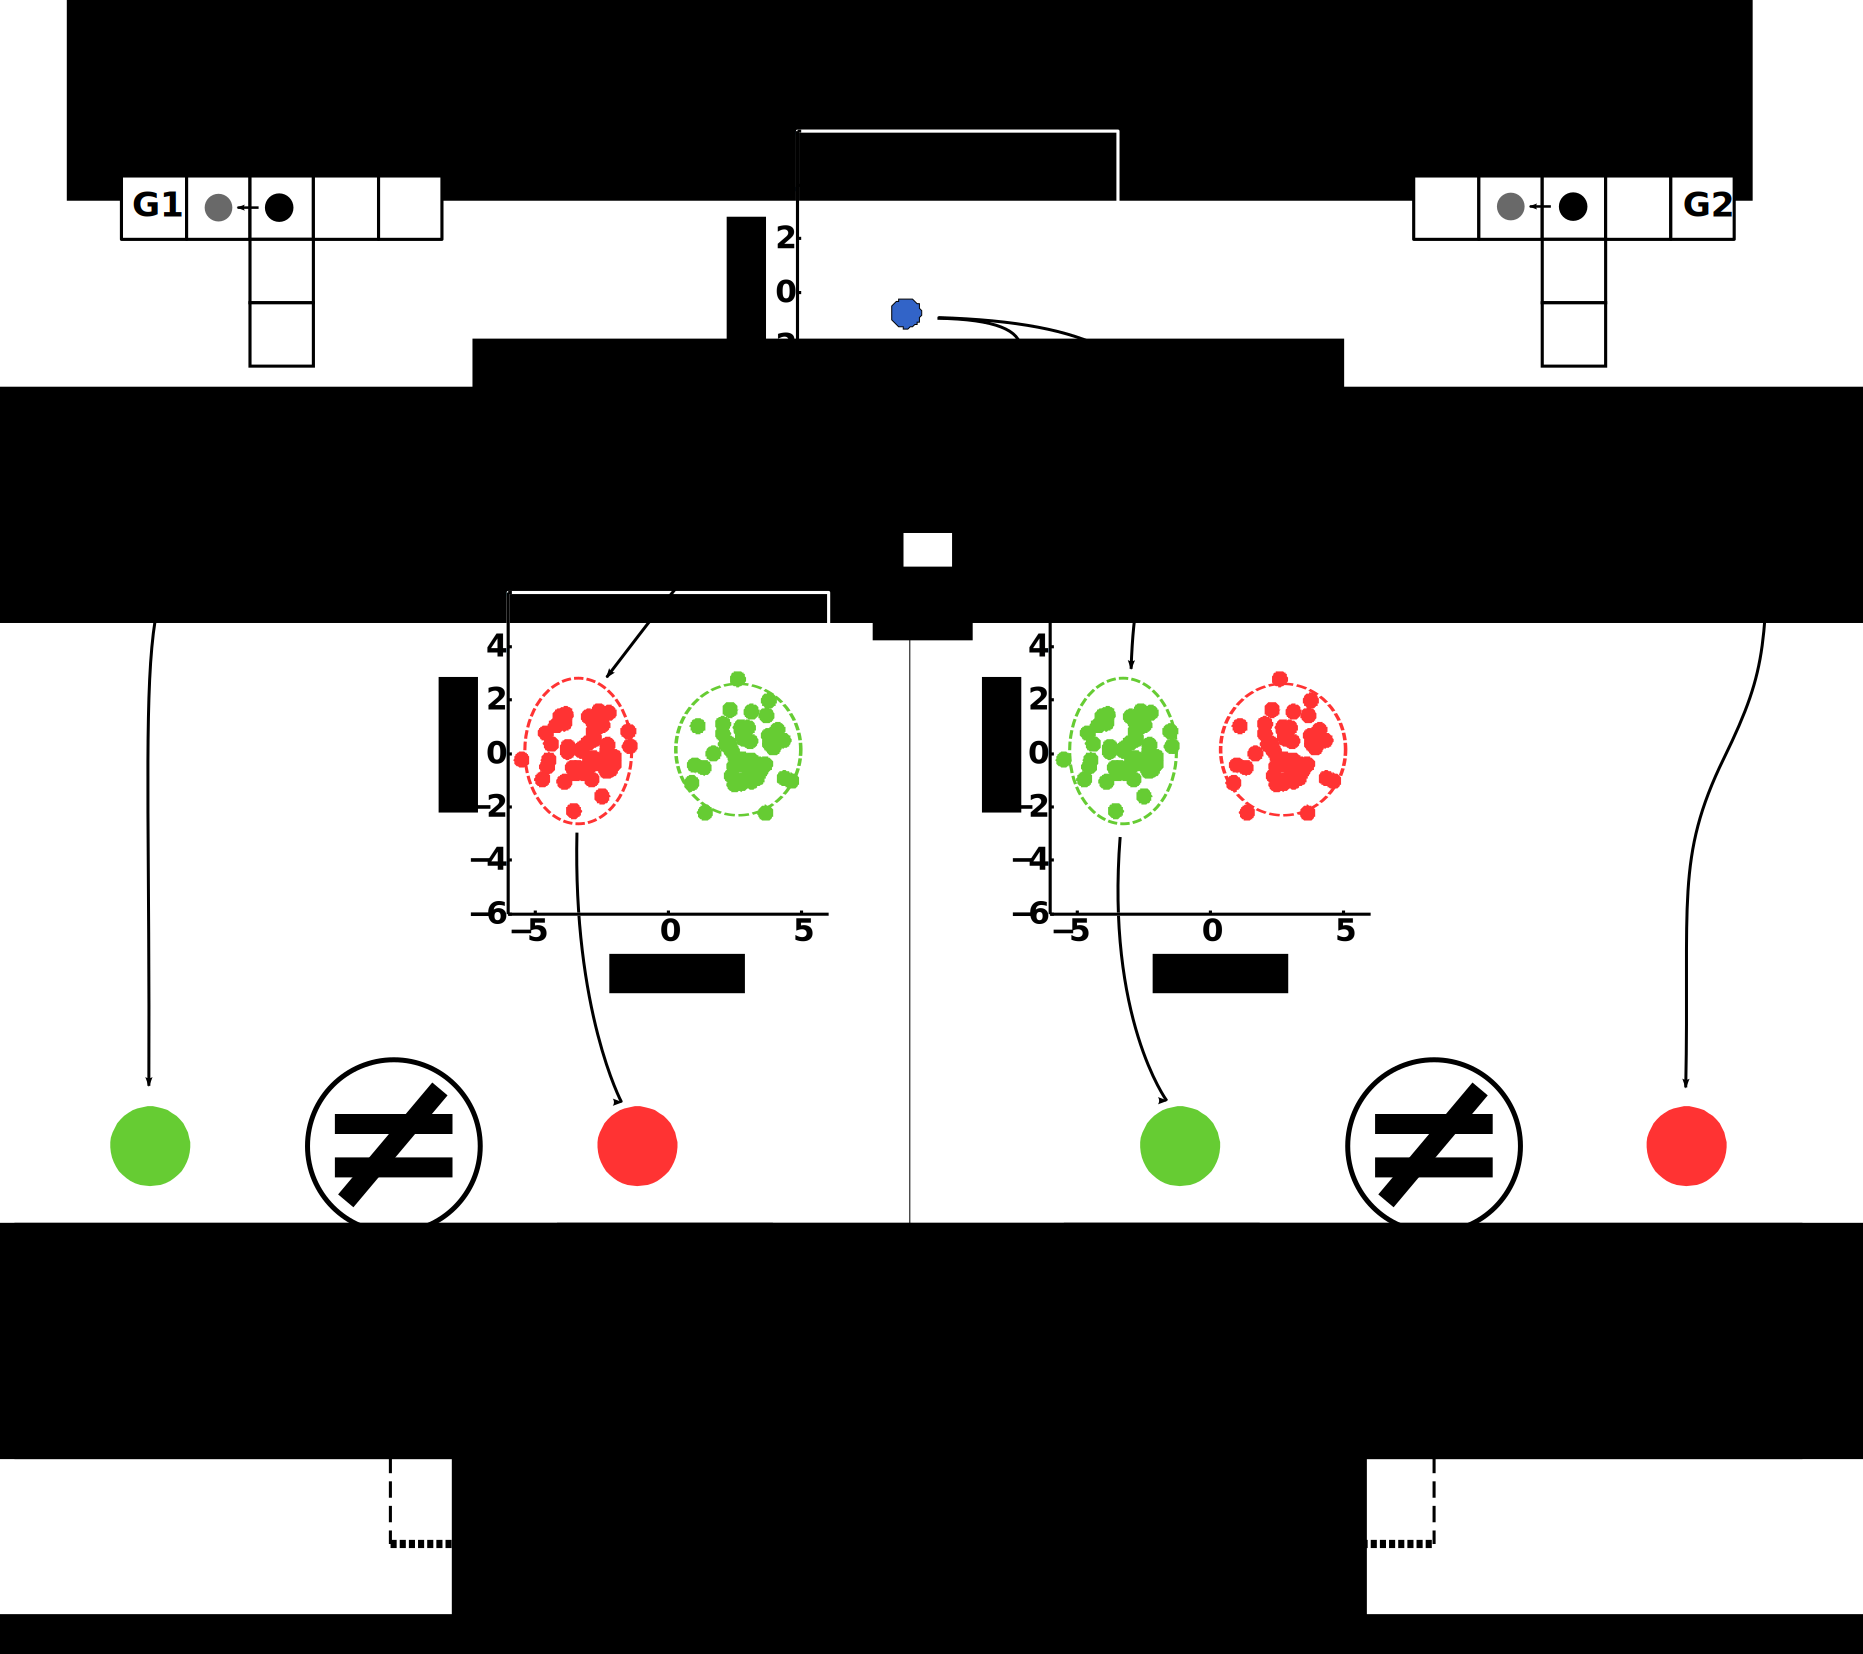
\includegraphics[width=\threeplanningwidth\columnwidth]{\visualspdf/planning/planning_right_left_expected_unmatched.pdf}
  \caption{Matching between expected labels and the prediction of a teaching signal sample on the left side of the feature space for the two hypothesis if the agent performs action left in state 3 and the two hypothesis currently have a symmetric interpretation of signals from Figure~\ref{fig:planningrightleft}. Both hypothesis agree that the label associated to a signal on the left side of the feature space does not match with the label predicted given the frame and the state-action pair considered. Therefore there is no uncertainty associated to this state-action pair and the agent should not select action left in order to disambiguate between hypothesis.}
  \label{fig:uncertaintymeaningrightleftexpectedright}
\end{figure}


However for action down, the two hypothesis disagree on whether such signals are expected or not given the state-action pair considered. As depicted in Figure~\ref{fig:uncertaintymeaningrightleftunexpectedright}, when selecting action down in state 3 and if the user sends a signal in the right part of the feature space, hypothesis 1 expects a signal of meaning ``incorrect'', and the teacher signal is classified as being of class ``correct''. And hypothesis 2 expects a signal of meaning ``incorrect'' and the teacher signal is classified as being of class ``incorrect''. Therefore receiving this particular signal after taking action down in state 3 is not expected for hypothesis 1 but expected for hypothesis 2, there is high uncertainty.

\begin{figure}[!ht]
  \centering
  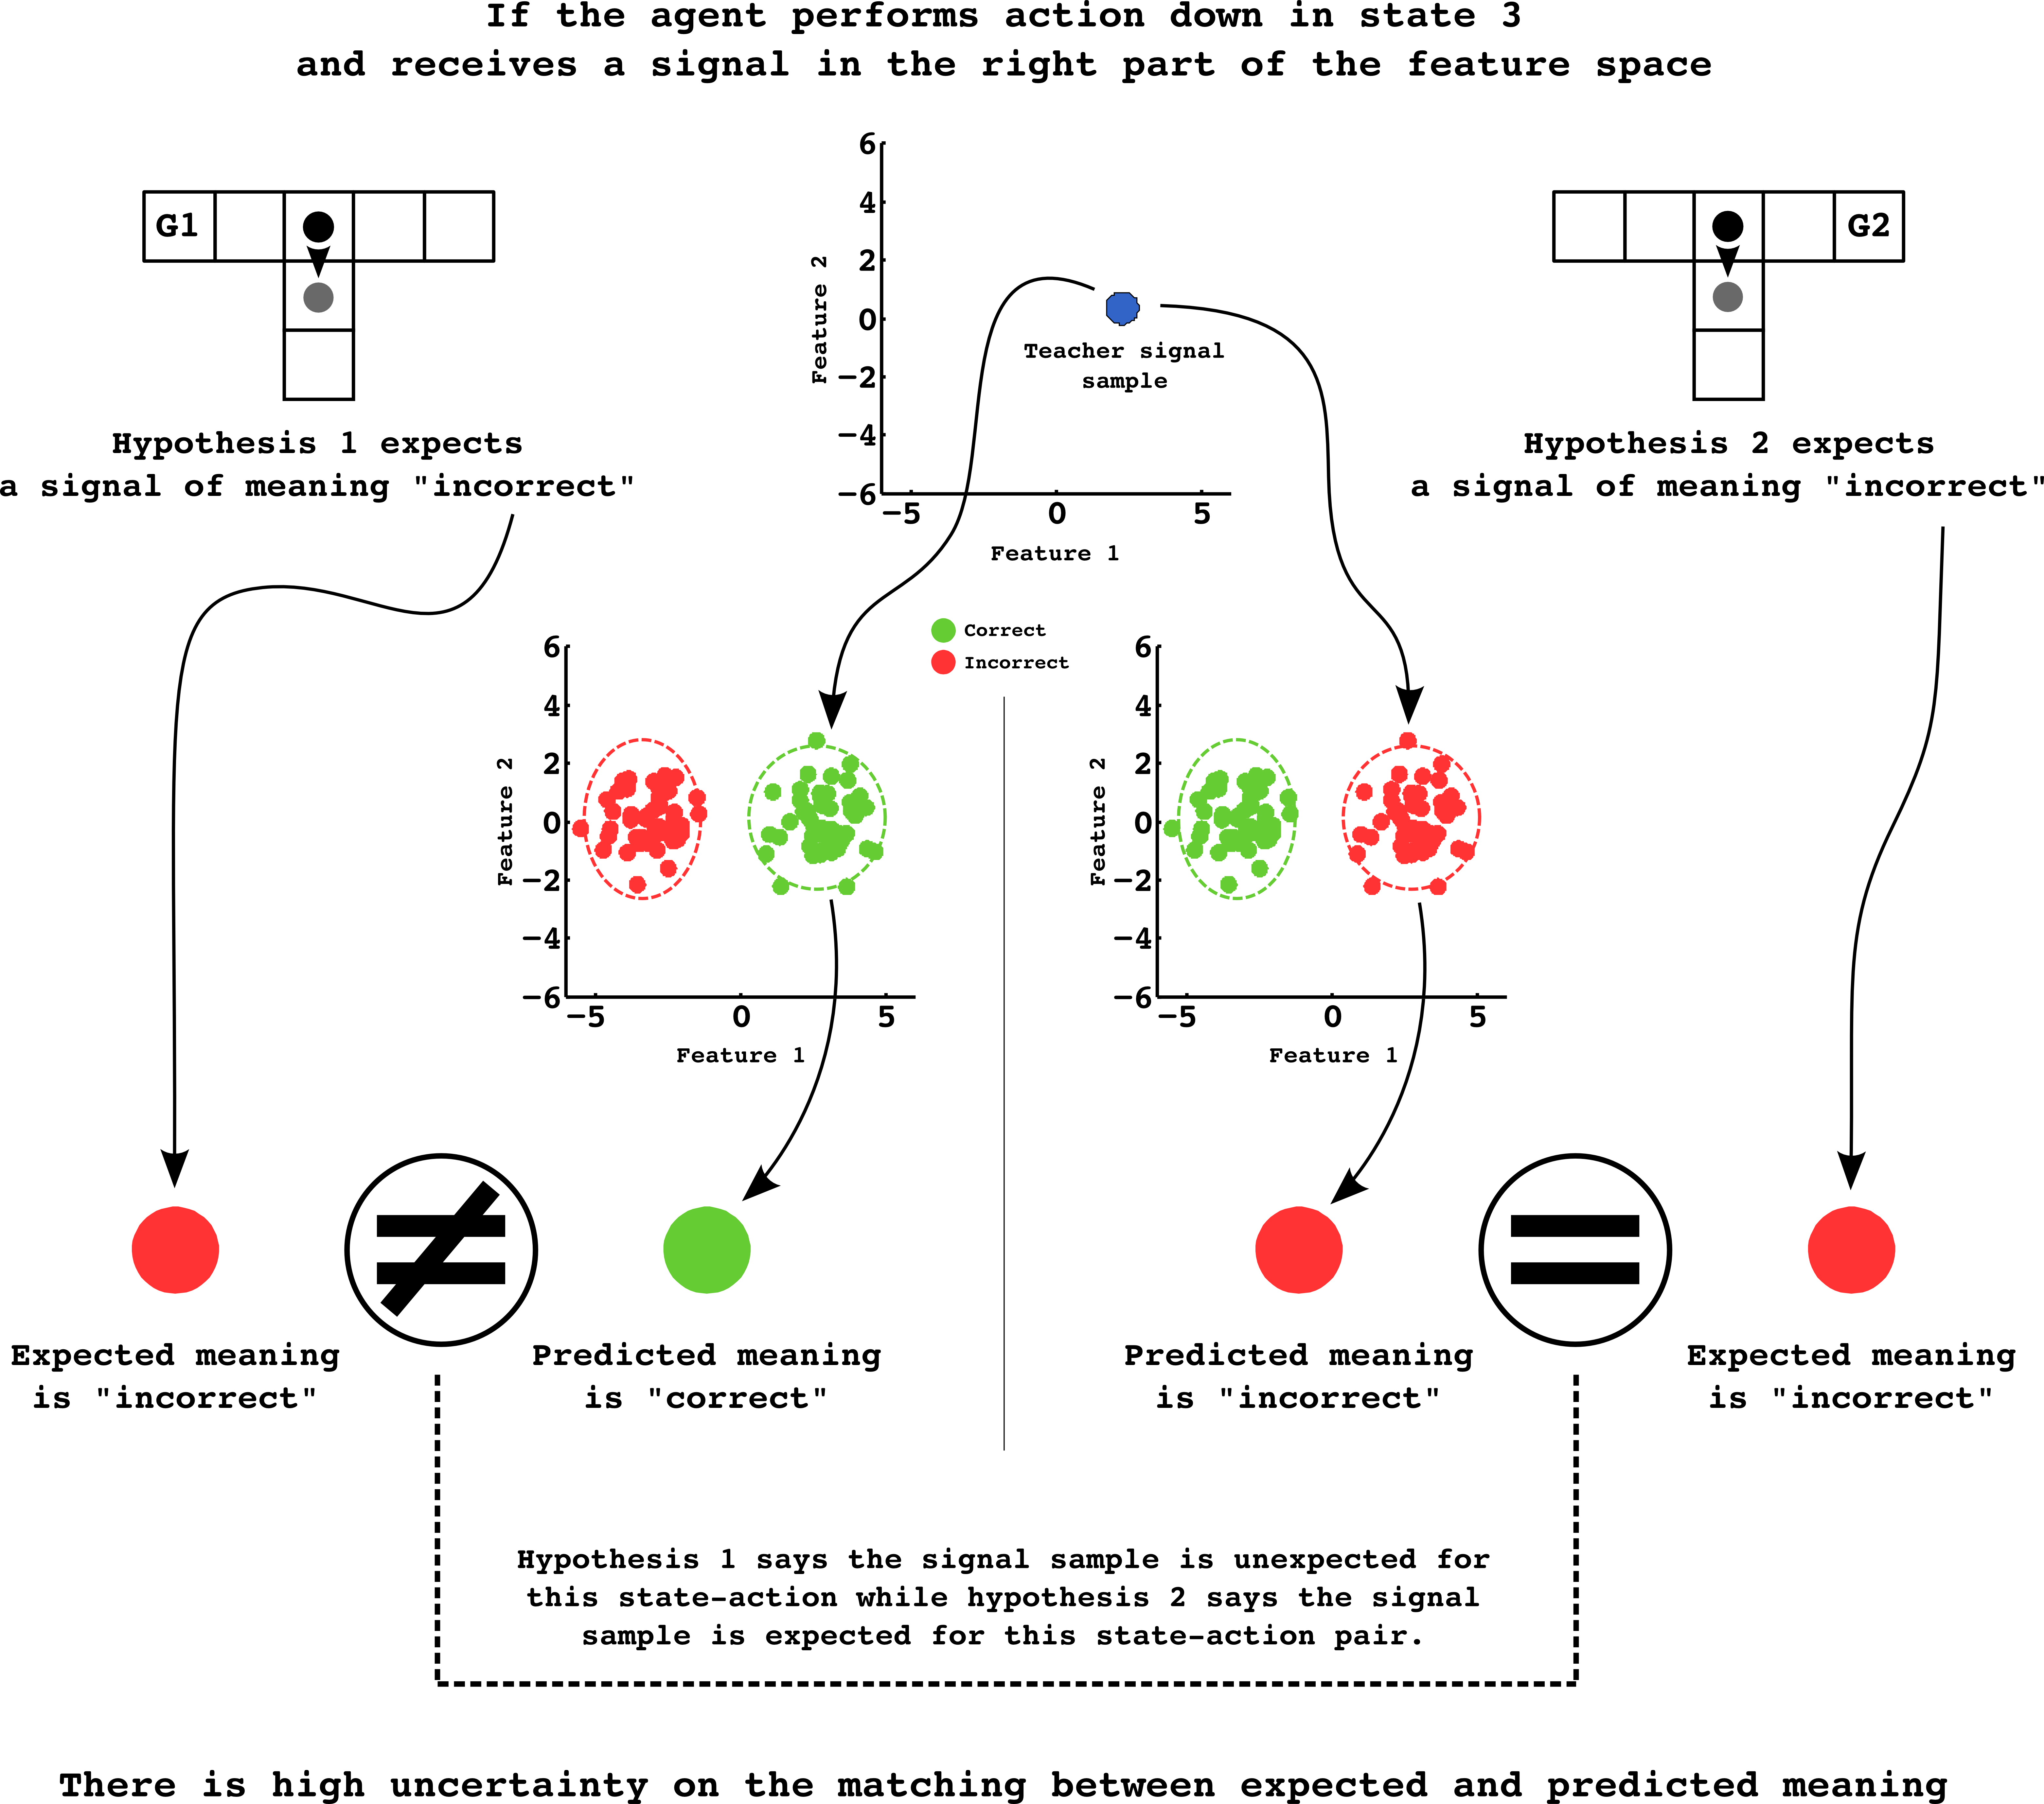
\includegraphics[width=\threeplanningwidth\columnwidth]{\visualspdf/planning/planning_right_left_unexpected_right_signal.pdf}
  \caption{Matching between expected labels and the prediction of a teaching signal sample on the right side of the feature space for the two hypothesis if the agent performs action down in state 3 and the two hypothesis currently have a symmetric interpretation of signals from Figure~\ref{fig:planningrightleft}. Hypothesis 1 says a signal on the right side of the feature space means ``correct'' which was not expected given the interaction frame, while hypothesis 2 expected a signal meaning ``incorrect'' and classify the signal as ``incorrect'' which is what was expected. Therefore there is high uncertainty associated to this state-action pair and the agent should better perform action down in order to disambiguate between hypothesis.}
  \label{fig:uncertaintymeaningrightleftunexpectedright}
\end{figure}

Similarly, as depicted in Figure~\ref{fig:uncertaintymeaningrightleftunexpectedleft}, considering a teaching signal on the left side of the feature space, if the agent performs action down in state 3, hypothesis 1 expects a signal of meaning ``incorrect'', and the teacher signal is classified as being of class ``incorrect''. And hypothesis 2 expects a signal of meaning ``incorrect'' and the teacher signal is classified as being of class ``correct''. Therefore receiving this particular signal after taking action down in state 3 is expected for hypothesis 1 but not expected for hypothesis 2, there is high uncertainty.

\begin{figure}[!ht]
  \centering
  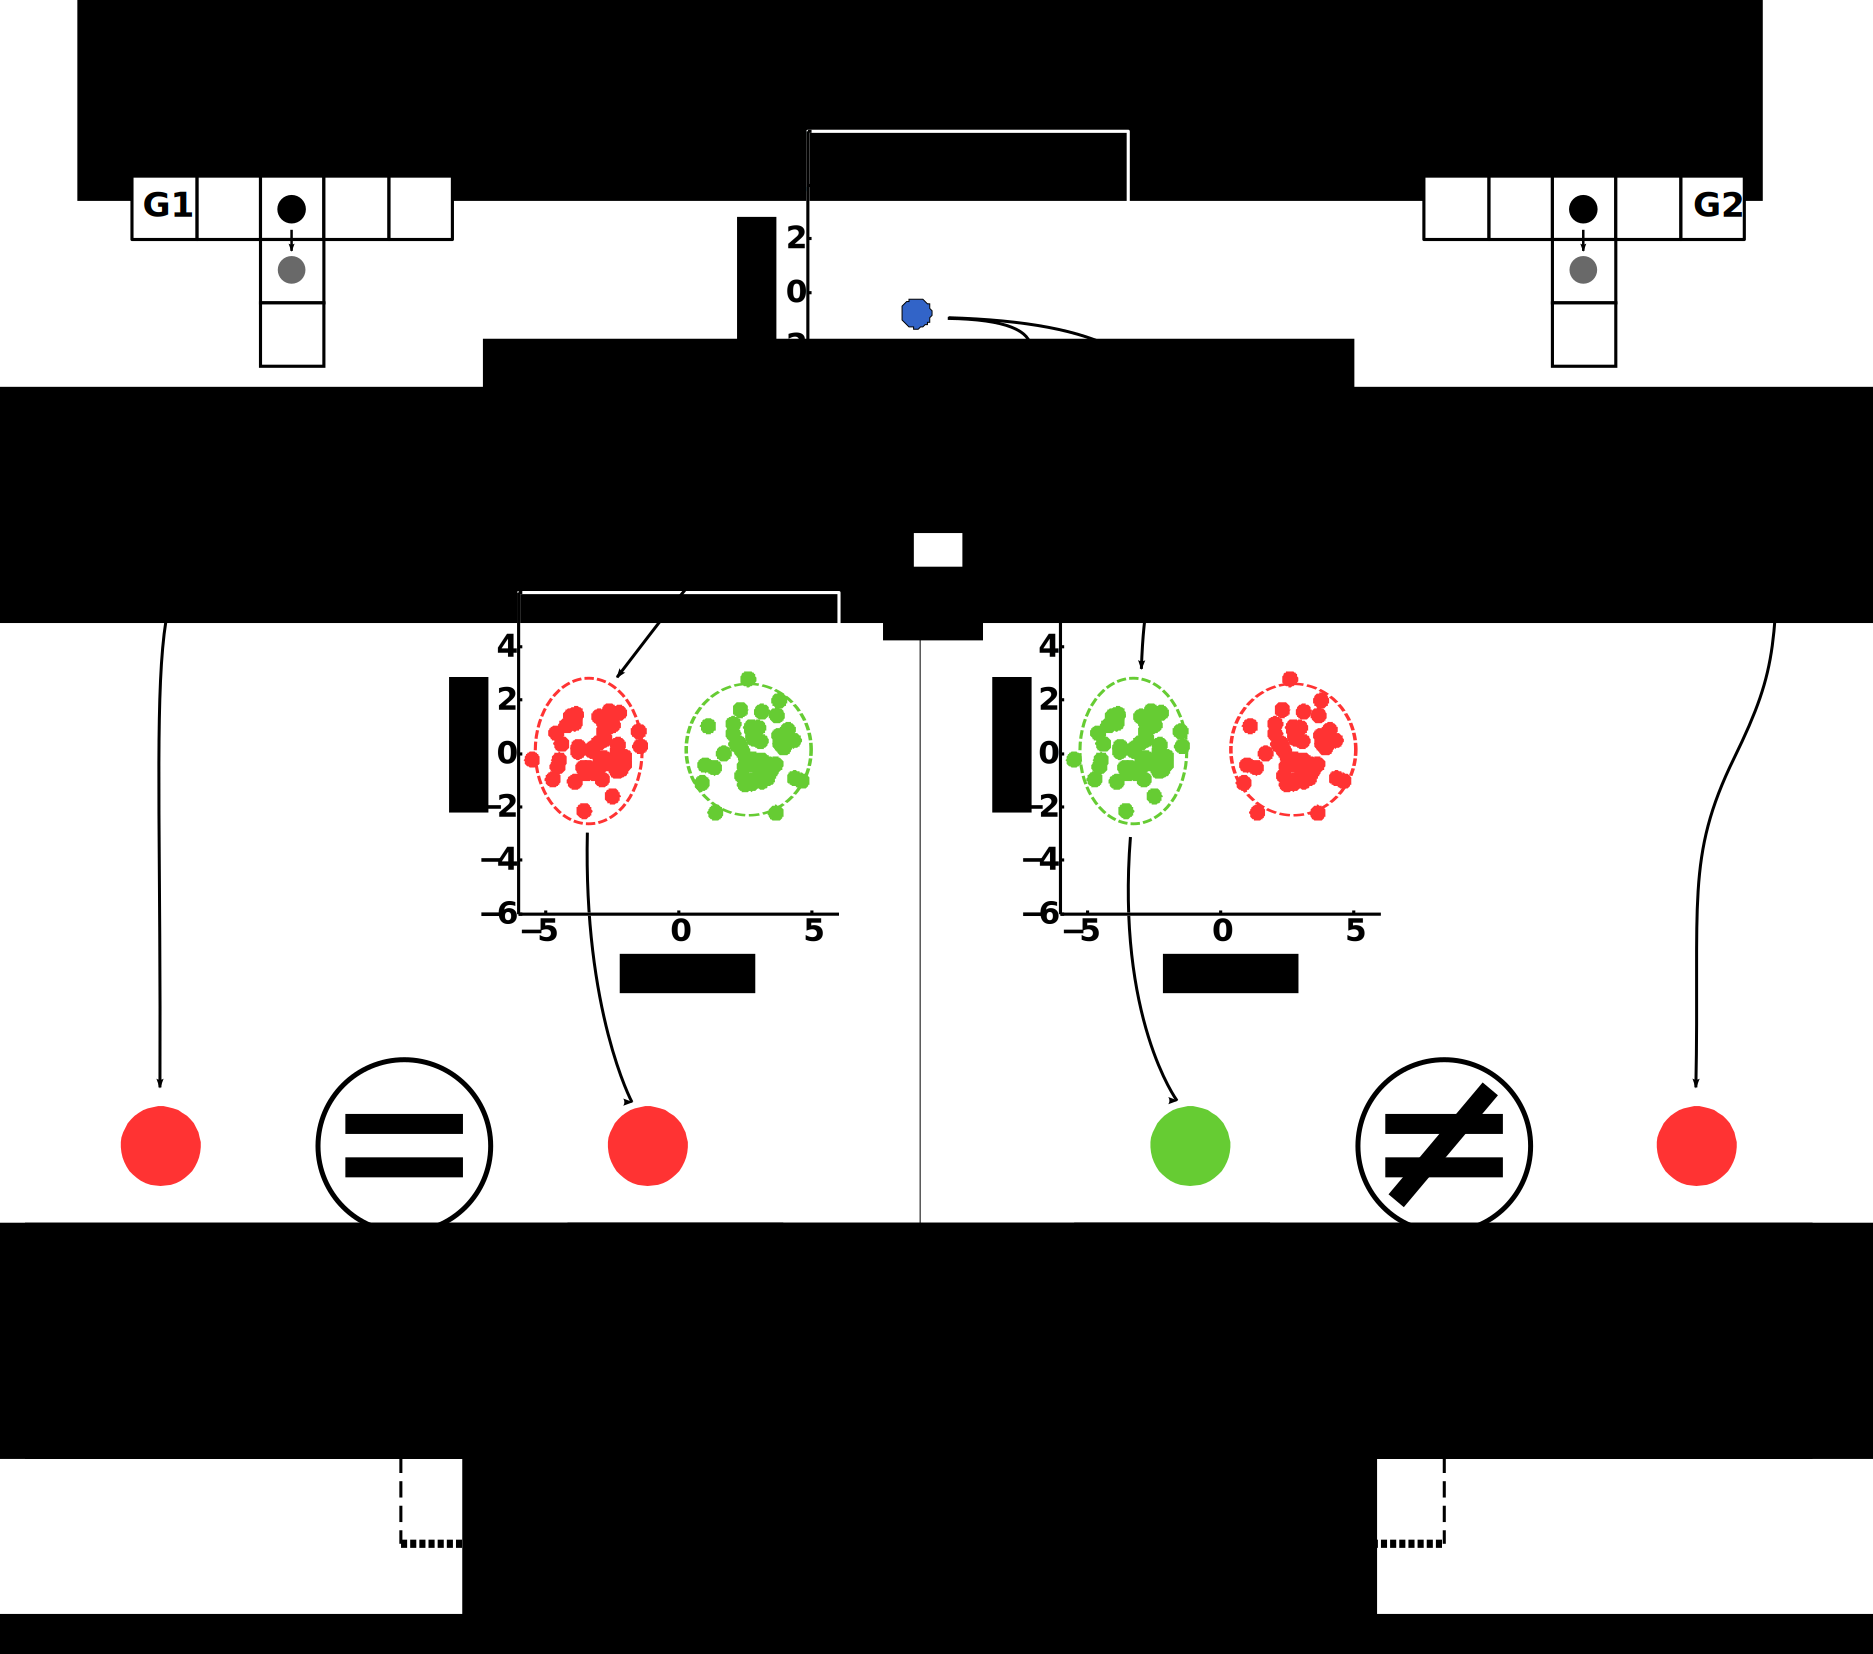
\includegraphics[width=\threeplanningwidth\columnwidth]{\visualspdf/planning/planning_right_left_unexpected_left_signal.pdf}
  \caption{Matching between expected labels and the prediction of a teaching signal sample on the left side of the feature space for the two hypothesis if the agent performs action down in state 3 and the two hypothesis currently have a symmetric interpretation of signals from Figure~\ref{fig:planningrightleft}. Hypothesis 1 says a signal on the left side of the feature space means ``incorrect'' which was expected given the interaction frame, while hypothesis 2 expected a signal meaning ``incorrect'' but classify the signal as ``correct'' which was not expected. Therefore there is high uncertainty associated to this state-action pair and the agent should better perform action down in order to disambiguate between hypothesis.}
  \label{fig:uncertaintymeaningrightleftunexpectedleft}
\end{figure}

This example holds for the case where the models between hypothesis are symmetric. For the situation in Figure~\ref{fig:planningupdown} where the two hypothesis have the same signal model, we report the same reasoning and illustration in appendix~\ref{appendix:uncertaintymeaning}. The example are similar to the one present above and illustrate that this way of measuring uncertainty holds for the situation in Figure~\ref{fig:planningupdown}.

To summarize, in order to estimate uncertainty between hypothesis for a given state-action pair, we can ask the system to classify some teaching signals $e$ and compute the probability that the predicted labels $l^c$ equals the expected labels $l^f$. Then, comparing the resulting joint probability between each hypothesis, if there is low variance in the estimate between hypothesis there is low uncertainty. Respectively, of the hypothesis disagree, i.e. if there is high variance, there is high uncertainty. 

This measure has the important advantage of using the exact same equation as the one used for computing the likelihood of each task (chapter~\ref{chapter:lfui:likelihood}). Additionally, we do not have to compute the similarity between continuous distribution. We only need to compute the predicted labels $l^c$ associated to the sampled signal $e$ once per hypothesis. Then, to compute the full uncertainty map for each state and action pair, we have to compare those predicted labels with the expected labels $l^f$ from each state-action pair and each hypothesis.

We note $J^{\xi_t}(s,a,e) = p(l^c = l^f | s, a, e, \theta_{xi_t}, \xi_t)$, which is Equation~\ref{eq:matchingoverfitting}) given the classifier $\theta_{\xi_t}$ associated to task $\xi_t$ and a particular state, action, and signal. We note $J^{\xi}(s,a,e)$ the vector $[J^{\xi_1}(s,a,e), \ldots, J^{\xi_T}(s,a,e)]$. and $W_{i}^{\xi} = [W^{\xi_1}, \ldots, W^{\xi_T}]$ the weights associated to each hypothesis. Such weight can be the one in presented in Equation~\ref{eq:probapairwise} or the probability from Equation~\ref{eq:probanormalize}.

The uncertainty of one state-action pair given a signal $e$ is computed as the weighted variance of the joint probabilities:

\begin{eqnarray}
U(s,a|e) = weightedVariance(J^{\xi}(s,a,e), W^{\xi})
\label{eq:planningOneSignal}
\end{eqnarray}

The uncertainty for a state-action pair is given by:
\begin{eqnarray}
U(s,a) & = & \int_{e} U(s,a|e) p(e) de
\end{eqnarray}
which we approximate by summing values of $U(s,a|e)$ for different signals $e$:
\begin{eqnarray}
U(s,a) & \approx & \sum_{e} U(s,a|e) p(e)
\label{eq:planning}
\end{eqnarray}
with $p(e)$ assumed uniform. 

The choice for the signal sample $e$ could be done randomly in the feature space but there is a high risk of taking non relevant samples (and practical computational problem for some classifiers). In practice, it is better to sample some signals from our past history of interaction. As the signals will be already observed by the classifiers, we may encounter overfitting problems which can be solved by using a cross validation procedure.

Our measure of uncertainty $U(s,a)$ will be higher when, for a given state-action there is an high incongruity of expectation between each hypothesis and according to the probability of each hypothesis. This measure is then used as a classical exploration bonus method. We provide an example of planning using this method in the following of this chapter.

\transition

Interestingly the two approaches proposed generalize over other active planning methods \cite{lopes2009active}, if the signal model is known, our equations reduces to the one presented in \cite{macl11simul}. For our first method relying on uncertainty of expected signal will be similar as a measure on expected meanings as all hypothesis will have identical signal models. For our second method, all classifiers will be the same and the resulting equation will no longer be dependent on signal $e$. As our uncertainty function combines uncertainty on both signal and task space, when former is known, the latter becomes the sole source of ambiguity.

\subsection{Why not building model first}

A usual question concerning Figure~\ref{fig:planningupdown}, is why don't we first select state-action pairs, where the interpretation is the same for all hypothesis? Indeed, this would allow to first build a database of known example and train a classifier which we could use to classify further teaching signals, as in a calibration procedure.

Obviously this is not always that easy, for example if we add a third hypothesis, it is not more possible to find actions whose interpretation are the same for all hypothesis. For our simple T world scenario, if we consider a third hypothesis G3 that is going in the bottom of the T trunk, neither the left and right actions (Figure~\ref{fig:planning3hyprightleft}), nor the up and down actions (Figure~\ref{fig:planning3hypupdown}) alone allow to have a unequivocal interpretation of the teaching signals. However taking all the actions (Figure~\ref{fig:planning3hyp}) will still make the difference between the hypothesis and highlight G1 has being the goal state the user as in mind.

In all the experiment presented in this thesis, there is no scenario where a state-action pair results in an unequivocal interpretation of the teaching signal. 

\begin{figure}[!ht]
  \centering
  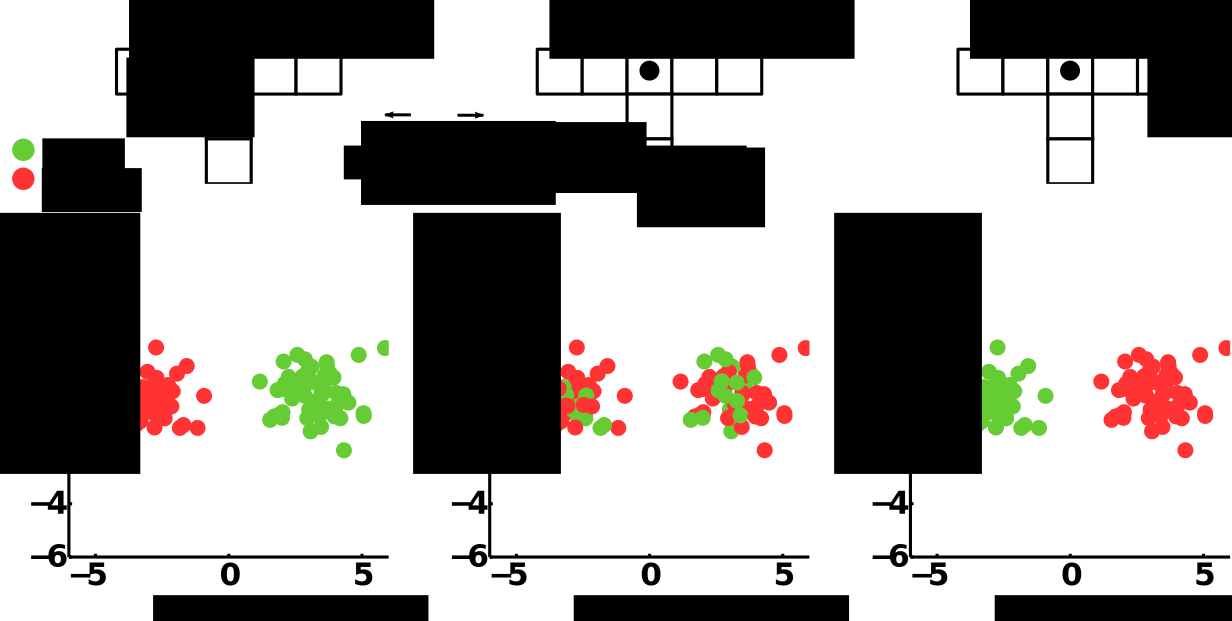
\includegraphics[width=\threetworldsize\columnwidth]{\visualspdf/planning/Tworld_feedback_3hyp_right_left.pdf}
  \caption{Interpretation hypothesis made by the agent according to G1 (left), G2 (right), and G3 (middle). The agent performs only left and right actions. The labels associated to G1 and G2 are symmetric while for G3 the labels are highly mixed. Right and left actions to not allow to have a unequivocal interpretation of signal considering those three hypothesis. However right and left actions allow to discard hypothesis G3.}
  \label{fig:planning3hyprightleft}
\end{figure}

\begin{figure}[!ht]
  \centering
  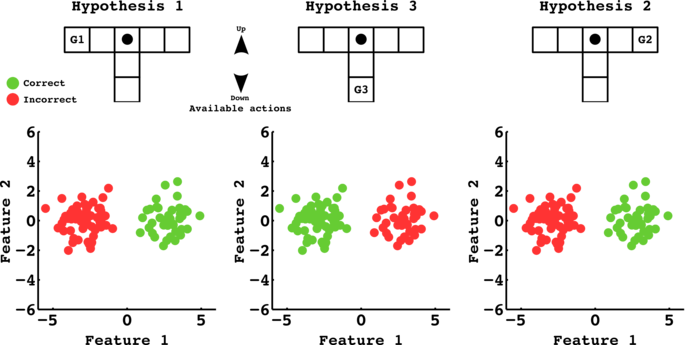
\includegraphics[width=\threetworldsize\columnwidth]{\visualspdf/planning/Tworld_feedback_3hyp_up_down_no_bump.pdf}
  \caption{Interpretation hypothesis made by the agent according to G1 (left), G2 (right), and G3 (middle). The agent performs only up and down actions. The labels associated to G1 and G2 are similar but he labels associated to G3 are symmetric. Up and down actions to not allow to have a unequivocal interpretation of signal considering those three hypothesis. Moreover u and down actions do not allow to discard any of the hypothesis.}
  \label{fig:planning3hypupdown}
\end{figure}

\begin{figure}[H]
  \centering
  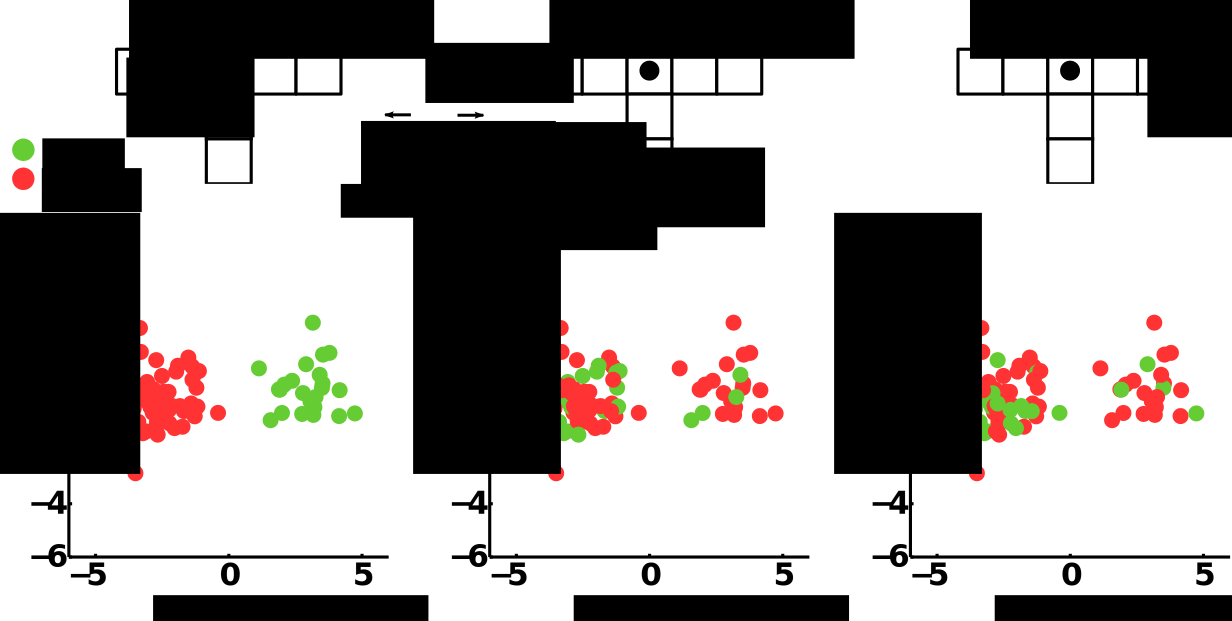
\includegraphics[width=\threetworldsize\columnwidth]{\visualspdf/planning/Tworld_feedback_3hyp.pdf}
  \caption{Interpretation hypothesis made by the agent according to G1 (left), G2 (right), and G3 (middle). The agent performs all possible actions. The labels associated to G1 are more coherent than with the spacial organization of the data than the labels associated to G2 and G3, which tells us G1 is the task the user has in mind.}
  \label{fig:planning3hyp}
\end{figure}

%%%%%%%%%%%%%%%%%%%%%%%%%%%%%%%%%%%%%%%%%%%%%%
%%%%%%%%%%%%%%%%%%%%%%%%%%%%%%%%%%%%%%%%%%%%%%
%%%%%%%%%%%%%%%%%%%%%%%%%%%%%%%%%%%%%%%%%%%%%%
%%%%%%%%%%%%%%%%%%%%%%%%%%%%%%%%%%%%%%%%%%%%%%
%%%%%%%%%%%%%%%%%%%%%%%%%%%%%%%%%%%%%%%%%%%%%%
\section{Method}
\label{chapter:planning:method}

In the subsequent analysis, we will considerer a reaching task where an agent live in a grid world and should learn which square the human user want the agent to go. We considered the teacher provides feedback for the actions taken by the agent. Our aim is to apply this algorithm to brain computer interaction, and we will use artificial dataset of different qualities and dimension to simulated EEG signals.

\subsection{World and Task}
We consider a 5x5 grid world, where an agent can perform five different discrete actions: move up, down, left, right, or a ``no move'' action. The user goal is to teach the agent to reach one (unknown to the agent) of the 25 discrete positions which represent the set of possible tasks. We thus consider that the agent has access to 25 different task hypothesis (one with goal location at each of the cells). We use \textit{Markov Decision Processes} (MDP) to represent the problem \cite{sutton1998reinforcement}. From a given task $\xi$, represented as a reward function, we can compute the corresponding policy $\pi^{\xi}$ using, for instance, Value Iteration \cite{sutton1998reinforcement}. The policies allow us to interpret the teaching signals with respect to the interaction protocol defined. For the current work we will consider the user is providing feedback on the agent action, and use the feedback frame function as define in Equation~\ref{eq:feedbackframe}.

\subsection{Signal properties and classifier}

We aim at applying this algorithm to error-related potentials (ErrPs) for EEG-based BCI applications. These signals are generated in the user's brain after s/he assesses actions performed by an external agent \cite{chavarriaga2010learning}, where correct and erroneous assessments will elicit different brain signals. Past approaches have already demonstrated that these signals can be classified online with accuracies of around 80\% and translated into binary feedback, thanks to a prior calibration session that lasts for 30-40 minutes \cite{chavarriaga2010learning, iturrate2013task}.

Following the literature \cite{blankertz2010single}, we will model the signals using independent multivariate normal distributions for each class, $\mathcal{N}(\mu_c, \Sigma_c), \mathcal{N}(\mu_w, \Sigma_w)$. With $\theta$ the set of parameters $\{\mu_c, \Sigma_c,\mu_w, \Sigma_w\}$. Given the high dimensionality of the problem we will also need to regularize. For this we apply shrinkage to the covariance matrix ($\lambda = 0.5$) and compute the value of the marginal pdf function using a noninformative (Jeffrey's) prior [\cite{gelman2003bayesian}, p88]:

\begin{eqnarray}
p(e|l, \theta) & = & t_{n-d}(e | \mu_l,\frac{\Sigma_l (n+1)}{n(n-d)})
\label{eq:prior}
\end{eqnarray}

where $\theta$ represents the ML estimates (mean $\mu_l$ and covariance $\Sigma_l$ for each class $l$) required to estimate the marginal under the Jeffreys prior, $n$ is the number of signals, and $d$ is the dimensionality of a signal feature vector.

\subsection{Task Achievement}

We will use Equation~\ref{eq:matchingfiltercrossvalidation} to compute the likelihood of each task using a 10 fold cross-validation to compute the confusion matrix. It implies we train 250 classifiers at each iteration. To compute the probability of each task, we will rely on the minimum of pairwise normalized likelihood measure as defined in Equation~\ref{eq:probapairwise}.

A task is considered completed when the confidence level $\beta$ as been reached for this task and the agent is located at the task associated goal state. If the state is the one intended by the user it is a success. Whatever the success or failure of the first task, the user selects a new goal state randomly, the agent resets task likelihoods, propagates the believed labels, and teaching starts again. At no point the agent has access to a measure of its performance, it can only refer to the unlabeled feedback signals from the user.

\subsection{Simulated teaching signals}

We analyze our algorithm using artificial datasets. The goal of this evaluation was to analyze the feasibility of learning a task from scratch in a 5x5 grid world. The artificial dataset was composed of two classes, with 1000 examples per class. Each example was generated by sampling from a normal distribution with a covariance matrix of diagonal 1 and mean selected randomly. The datasets were generated while varying two factors: (i) the dimensionality of the data, where 2, 5, 10 and 30 features were tested; and (ii) the quality of the dataset, measured in terms of the ten-fold accuracy the classifier would obtain. Some two dimensional classifier of different quality are shown in Figure~\ref{fig:datasetsquality}.

\begin{figure}[!ht]
  \centering
      \includegraphics[width=\columnwidth]{\visualspdf/worlds_and_datasets/dataset_qualities.pdf}
      \caption{Artificial dataset generated generated by sampling from a normal distribution with a covariance matrix of diagonal 1 and mean selected randomly. From left to right, we show dataset of increasing quality as measured by a 10 fold cross-validation train-test procedure using a Gaussian classifier.}
    \label{fig:datasetsquality}
\end{figure}


\subsection{Evaluation scenarios}

Using the datasets generated, three different evaluations were performed: (i) the goodness of our proposed planning strategy versus a) random action selection, b) greedy action selection, and c) a task-only uncertainty based method; (ii) the time required by the agent to learn the first task (i.e. to reach the first target), and (iii) the number of tasks that can be reached correctly and incorrectly in 500 iterations.

\subsection{Settings}

We used $\alpha = 0.1$, $\beta = 0.9$. For dataset of dimension $d$, we started computing likelihoods after $d+10$ steps as equation \ref{eq:prior} requires at least $d+1$ samples and to allow for cross validation. For the planning (Eq. \ref{eq:planning}) we selected randomly $20$ signals from $D_M$.


%%%%%%%%%%%%%%%%%%%%%%%%%%%%%%%%%%%%%%%%%%%%%%
%%%%%%%%%%%%%%%%%%%%%%%%%%%%%%%%%%%%%%%%%%%%%%
%%%%%%%%%%%%%%%%%%%%%%%%%%%%%%%%%%%%%%%%%%%%%%
%%%%%%%%%%%%%%%%%%%%%%%%%%%%%%%%%%%%%%%%%%%%%%
%%%%%%%%%%%%%%%%%%%%%%%%%%%%%%%%%%%%%%%%%%%%%%
\section{Results}

We present most of the results in terms of the quality of the dataset, measured as the ten-fold classification accuracy that a calibrated signal classifier would obtain. Each simulation was run 100 times using different sampled datasets, and their associated box plots were computed. For each boxplot, colored bars show the interquartile range (between 25th and 75th percentile), and the median and the mean are marked as a horizontal line and a colored dot respectively. Additionally, the two whiskers show the 5th and 95th percentiles, black crosses are outliers. 

The first objective is to study the impact of the exploration approach proposed in this section. The second is to evaluate performances and robustness with respect to the dimension and the quality of each dataset.

\subsection{Planning methods}

Figure~\ref{fig:artificialplanning} compares the number of steps (with maximum values of 500 steps) needed to identify the first task when learning from scratch with different planning methods. Following the most probable task (i.e. going greedy) does not allow the system to explore sufficiently. On the contrary, our proposed planning method leads the system towards regions that maximize disambiguation among hypotheses. Furthermore, it also performs better than assessing uncertainty on the meaning space only. Given these results, the remainder of this section will only consider our planning method.

\begin{figure}[!ht]
  \centering
      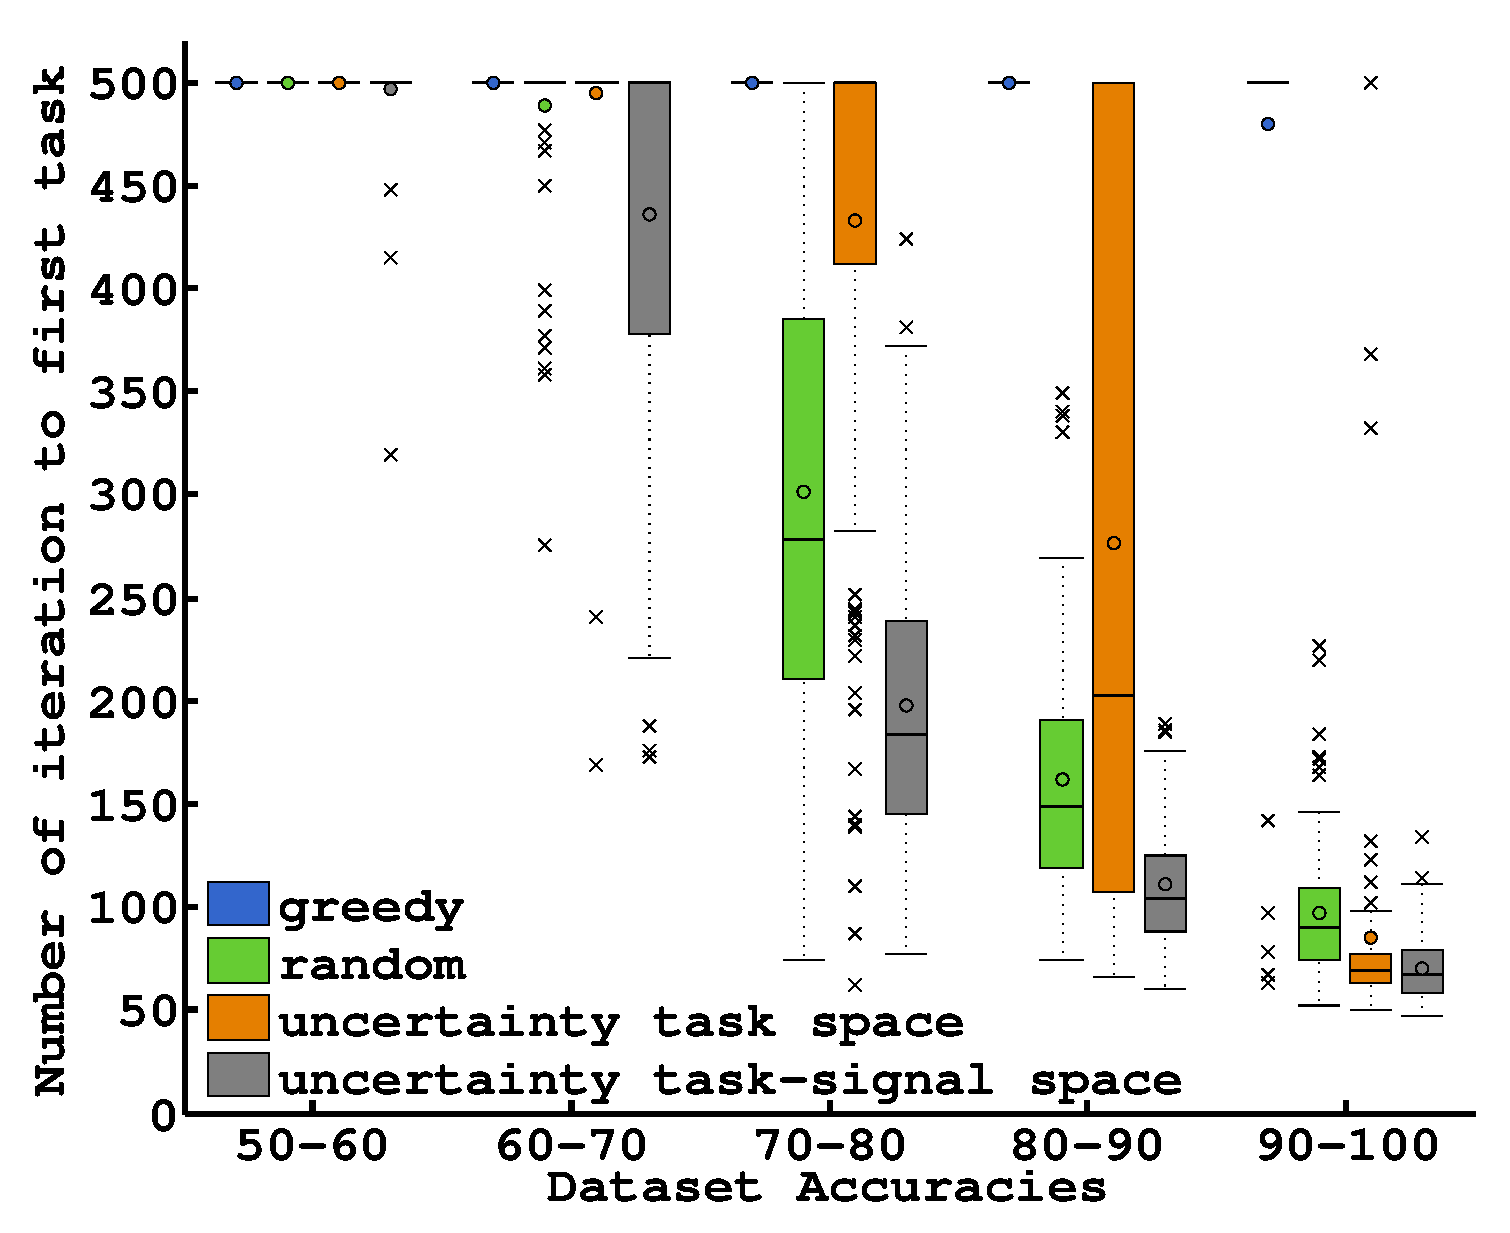
\includegraphics[width=\plotsize\columnwidth]{\imgpath/plot_artificial_planning.eps}
      \caption{Number of steps to complete first task, comparison of different exploration methods with 30 dimensional artificial data. When learning from scratch, planning upon uncertainty in both task and signal space performs better than relying only on task uncertainty. Greedy action selection rarely disambiguates between hypothesis.}
    \label{fig:artificialplanning}
\end{figure}

As explained in section~\ref{chapter:planning:how}, the machine needs to collect two types of information, some about the true underlying model (Fig.~\ref{fig:planningupdown} and some to differentiate between hypotheses (Fig.~\ref{fig:planningrightleft}. The properties of the grid world make the random strategy quite efficient at collecting those two types of information. The differences between planning methods should be more evident when navigating a complex maze since our method allows to plan in order to collect the type of information we need. 

We will present a small study on how different world properties affect the learning efficiency in chapter~\todo{reference this here once written}. 

Also, we note that all planning methods were switched to pure exploitation (greedy) once the confidence level was reached. Therefore the performance in Figure~\ref{fig:artificialplanning} compares the ability of the different methods to discriminate between different task hypotheses, not their ability to solve the task itself.

\subsection{Dimensionality}

Figure~\ref{fig:firstArtificial} compares the number of steps (with maximum values of 500 steps) needed to identify the first task when learning from scratch with different dimensionality of datasets. The convergence speed is only slightly affected by the features dimensionality. On the other hand, the dataset quality (measured in terms of its associated ten-fold accuracy) is the main cause of performances decay. Furthermore, for those datasets with accuracies between $50\%$ and $60\%$, the system is not able to identify a task with confidence after 500 steps. This is the expected behavior as for such dataset (see Figure~\ref{fig:datasetsquality} left), none of the hypothesis is able to find a classifier of good enough accuracy and should therefore not take any decision.

\begin{figure}[!ht]
  \centering
      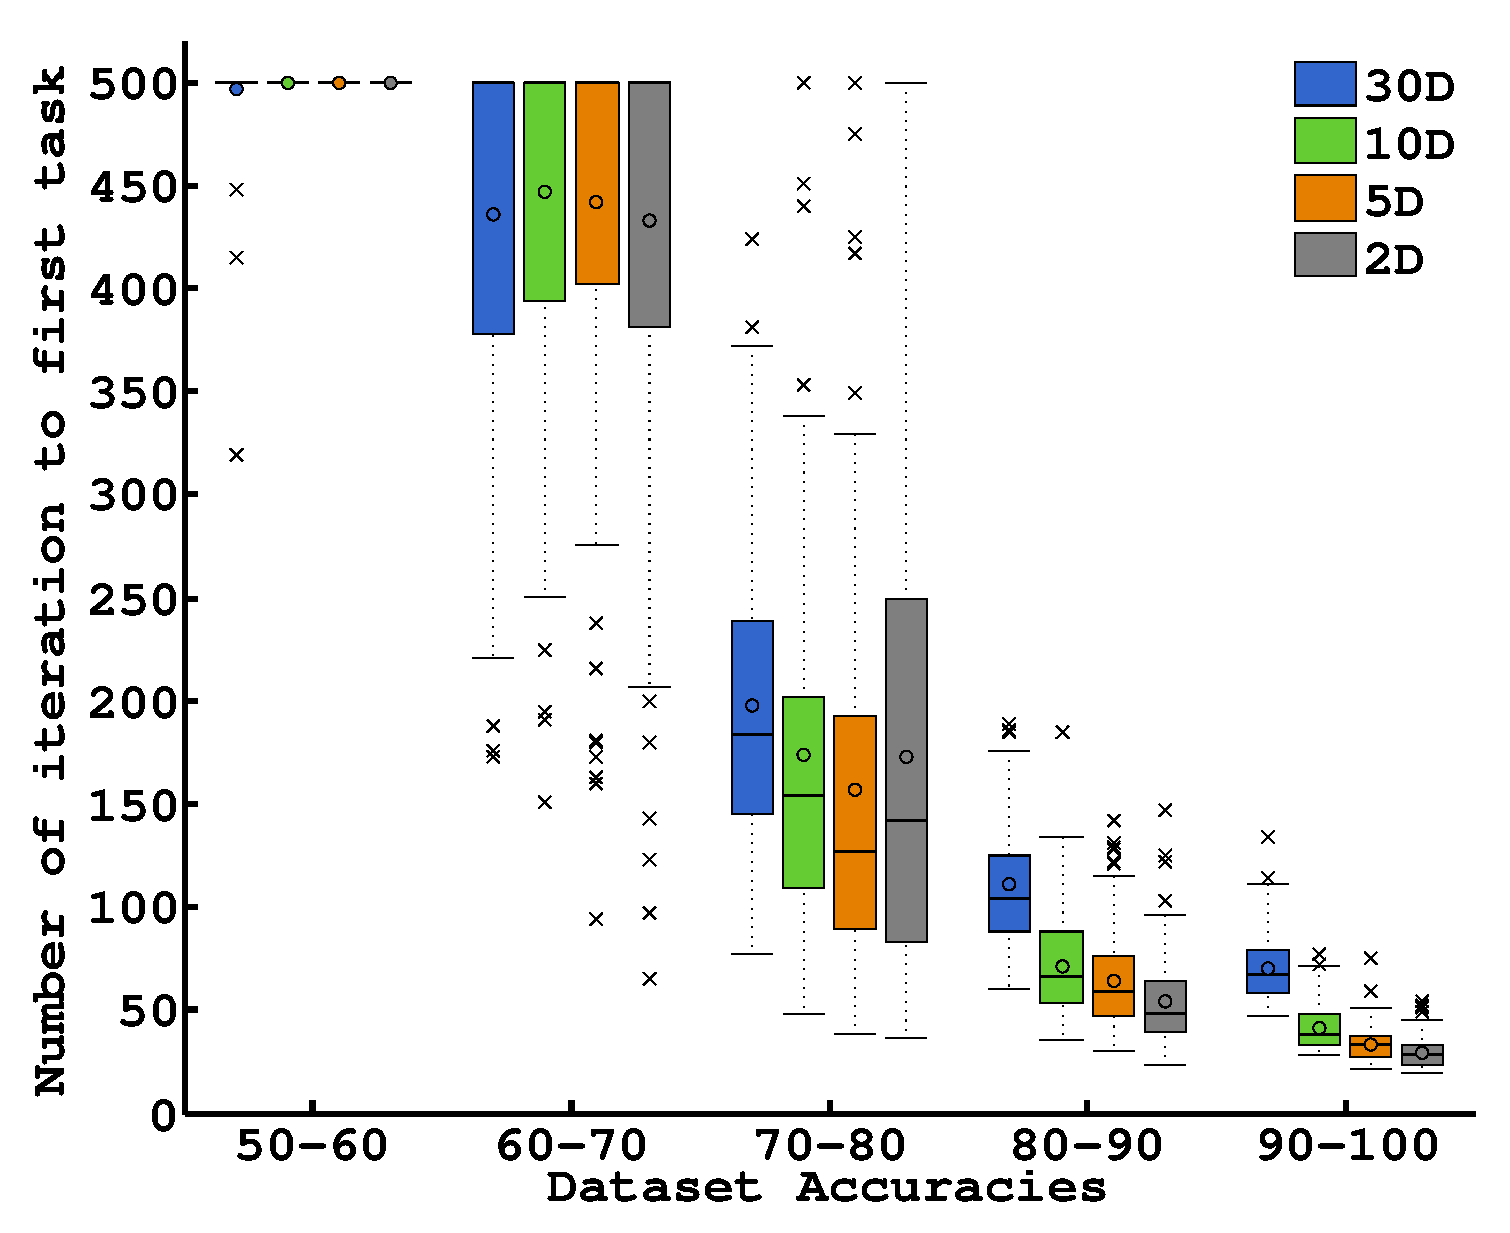
\includegraphics[width=\plotsize\columnwidth]{\imgpath/plot_artificial_firstconf.eps}
      \caption{Number of steps to complete first task using artificial data. Under 60 percent accuracy, the confidence threshold cannot be reached in 500 steps. The dataset qualities, more than their dimensionality, impact the learning time.}
      \label{fig:firstArtificial}
\end{figure} 

\subsection{Reuse}

Once the first task is completed, a new one is selected randomly. Figure~\ref{fig:nCorrectArtificial} compares the number of tasks that can be achieved in 500 steps. As expected, the lower the quality of the data, the less number of task can be completed. With dataset accuracies higher than $90\%$ we can achieve more than 30 tasks on average.

\begin{figure}[!ht]
    \centering
    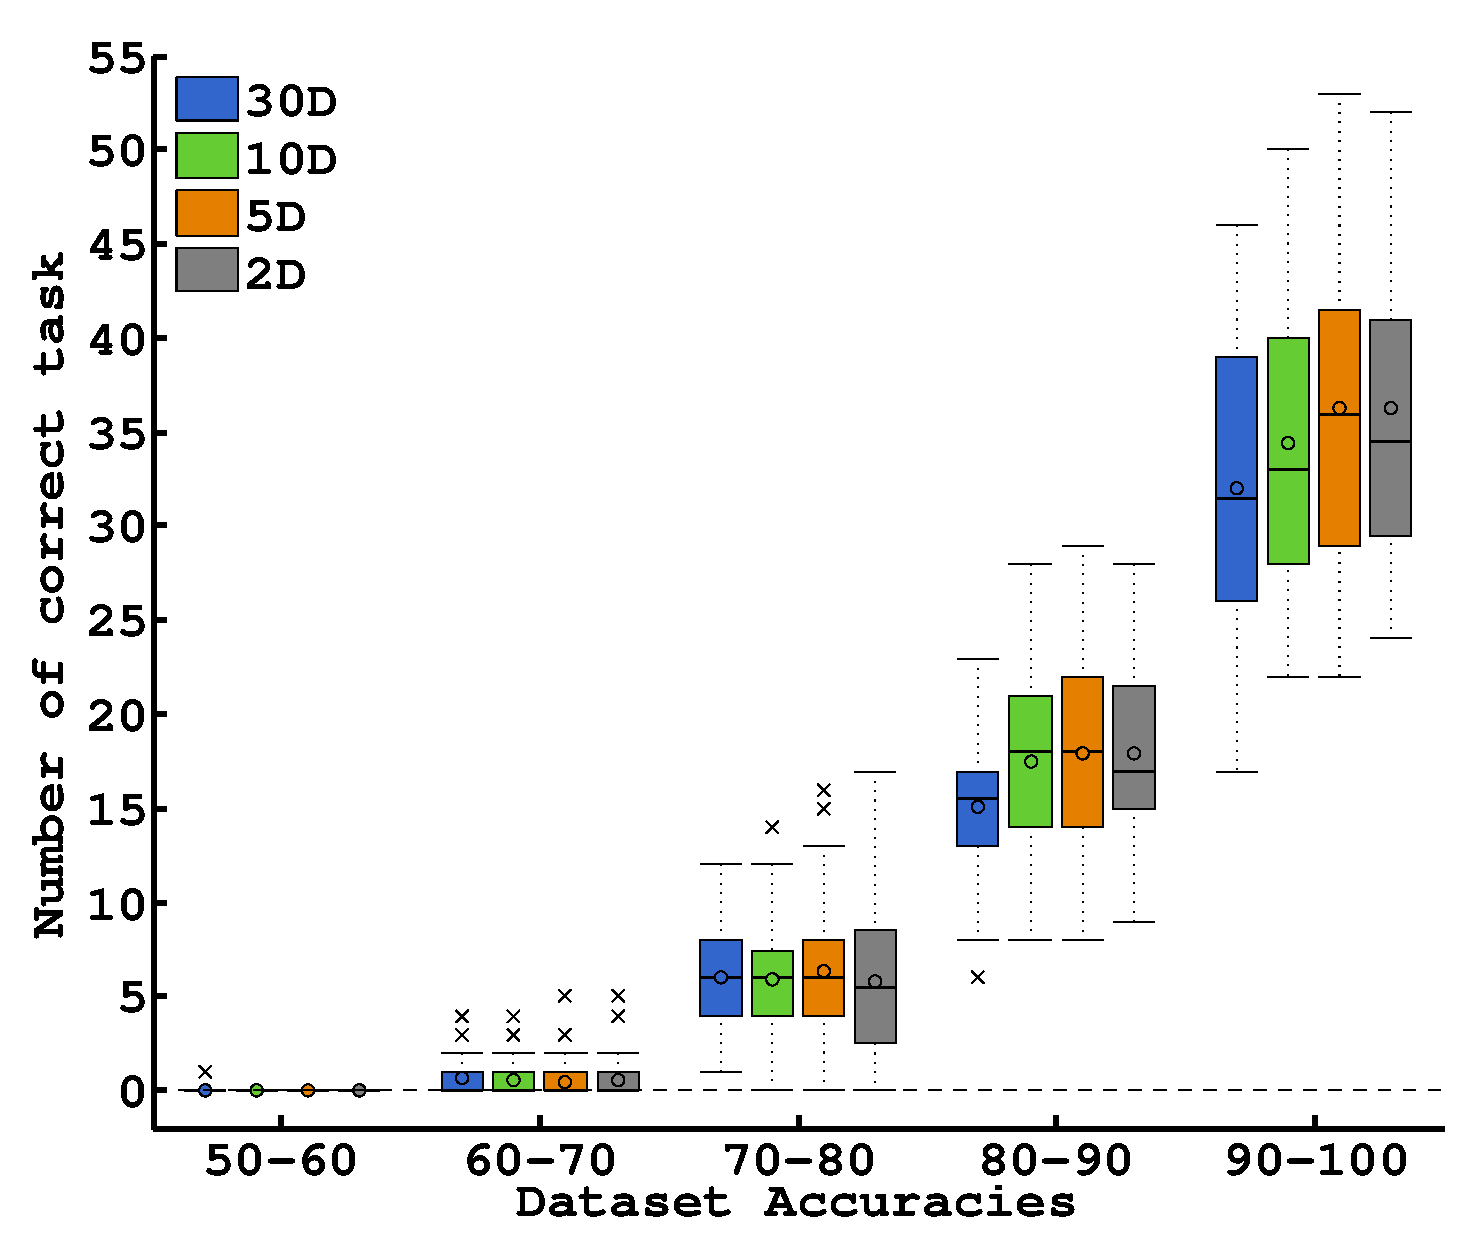
\includegraphics[width=\plotsize\columnwidth]{\imgpath/plot_artificial_nCorrect.eps}
    \caption{Number of tasks correctly achieved in 500 steps, artificial data. Quality of dataset impacts the number of task identified in 500 steps as more evidence should be collected to reach the confidence threshold.}
    \label{fig:nCorrectArtificial}
\end{figure} 

An important aspect of the proposed learning approach was that the first task learned was always the correct one. We reported only 9 erroneous estimations across all simulated experiments (5 in the 70-80 group and 4 in the 80-90 group).


\transition

We have presented a planning method that allowed to speed up the time needed to identify the correct task from unlabeled teaching signals. This method was based on assigning an uncertainty value to each state-action pair and have the agent reaching for the most uncertain one in order to disambiguate faster between the hypothesis. We identified two source of uncertainty, one coming from the expected meanings and the other coming from the signal model attributed to each task hypothesis. We presented two methods to measure this uncertainty. The first method measures the uncertainty on the expected signals between each hypothesis. The second method rely on sampling some teaching signals and asking each hypothesis if this signal is expected or not.

We now want to apply this algorithm to a more concrete scenario. In next chapter we present a brain computer interaction scenario following the experimental scenario presented in this section. But instead of using artificial data, we will investigate own our algorithm scale to real EEG feature first in simulation and then in online experiments with real subjects. The application of this work to BCI is a joint collaboration with I{\~n}aki Iturrate and Luis Montesano.
